
%%%%%%%%%%%%%%%%%%%%%%%%%%%%%%%%%%%%%%%%%%%%%%%%%%%%%%%%%%%%%%%%%%
%
% Custom UNSW-provided thesis style
%
%%%%%%%%%%%%%%%%%%%%%%%%%%%%%%%%%%%%%%%%%%%%%%%%%%%%%%%%%%%%%%%%%%

\documentclass[honours,12pt]{UNSWthesis}

\usepackage{amsfonts}
\usepackage{amssymb}
\usepackage{amsthm}
\usepackage{latexsym,amsmath}
\usepackage{bm}
\usepackage{bbm}
\usepackage{graphicx}
\usepackage{afterpage}
\usepackage{accents}
\usepackage{comment}

% Package for linking and referencing
\usepackage[bookmarksopen]{hyperref}
\hypersetup{
    bookmarksopen=true,
    bookmarksnumbered,
    colorlinks=true,
    citecolor=blue,
    filecolor=blue,
    linkcolor=blue,
    urlcolor=blue
}
\newcommand*{\Appendixautorefname}{Appendix}

% Package for bibliography
\usepackage[
    backend=biber,
    style=numeric,
    sorting=none
]{biblatex}

\addbibresource{references.bib}

% Package for bringing in figures generated by tikzdevice
\usepackage{tikz}

% A simple LaTeX macro to add an equation reference to an
% align* environment
% Courtesy of https://tex.stackexchange.com/a/42728
\newcommand\numberthis{\addtocounter{equation}{1}\tag{\theequation}}

% Set table of contents depth to part,chapters,sections
\setcounter{tocdepth}{1}

% Macro for convergence in distribution
\newcommand{\Dconverge}{\overset{D}{\longrightarrow}}
\newcommand{\Pconverge}{\overset{P}{\longrightarrow}}

%%%%%%%%%%%%%%%%%%%%%%%%%%%%%%%%%%%%%%%%%%%%%%%%%%%%%%%%%%%%%%%%%
%
%  The following are some simple LaTeX macros to give some
%  commonly used letters in funny fonts. You may need more or less of
%  these
%
\newcommand{\R}{\mathbb{R}}
\newcommand{\Q}{\mathbb{Q}}
\newcommand{\C}{\mathbb{C}}
\newcommand{\N}{\mathbb{N}}
\newcommand{\F}{\mathbb{F}}
\newcommand{\PP}{\mathbb{P}}
\newcommand{\T}{\mathbb{T}}
\newcommand{\Z}{\mathbb{Z}}
\newcommand{\B}{\mathfrak{B}}
\newcommand{\BB}{\mathcal{B}}
\newcommand{\M}{\mathfrak{M}}
\newcommand{\X}{\mathfrak{X}}
\newcommand{\Y}{\mathfrak{Y}}
\newcommand{\CC}{\mathcal{C}}
\newcommand{\E}{\mathbb{E}}
\newcommand{\cP}{\mathcal{P}}
\newcommand{\cN}{\mathcal{N}}
\newcommand{\cS}{\mathcal{S}}
\newcommand{\A}{\mathcal{A}}
\newcommand{\ZZ}{\mathcal{Z}}
%%%%%%%%%%%%%%%%%%%%%%%%%%%%%%%%%%%%%%%%%%%%%%%%%%%%%%%%%%%%%%%%%%%%%
%
% The following are much more esoteric commands that I have left in
% so that this file still processes. Use or delete as you see fit
%
\newcommand{\bv}[1]{\mbox{BV($#1$)}}
\newcommand{\comb}[2]{\left(\!\!\!\begin{array}{c}#1\\#2\end{array}\!\!\!\right)
}
\newcommand{\Lat}{{\rm Lat}}
\newcommand{\var}{\mathop{\rm var}}
\newcommand{\Pt}{{\mathcal P}}
\def\tr(#1){{\rm trace}(#1)}
\def\Exp(#1){{\mathbb E}(#1)}
\def\Exps(#1){{\mathbb E}\sparen(#1)}
\newcommand{\floor}[1]{\left\lfloor #1 \right\rfloor}
\newcommand{\ceil}[1]{\left\lceil #1 \right\rceil}
\newcommand{\hatt}[1]{\widehat #1}
\newcommand{\modeq}[3]{#1 \equiv #2 \,(\text{mod}\, #3)}
\newcommand{\rmod}{\,\mathrm{mod}\,}
\newcommand{\p}{\hphantom{+}}
\newcommand{\vect}[1]{\mbox{\boldmath $ #1 $}}
\newcommand{\reff}[2]{\ref{#1}.\ref{#2}}
\newcommand{\psum}[2]{\sum_{#1}^{#2}\!\!\!'\,\,}
\newcommand{\bin}[2]{\left( \begin{array}{@{}c@{}}
				#1 \\ #2
			\end{array}\right)	}
%
%  Macros - some of these are in plain TeX (gasp!)
%
\newcommand{\be}{($\beta$)}
\newcommand{\eqp}{\mathrel{{=}_p}}
\newcommand{\ltp}{\mathrel{{\prec}_p}}
\newcommand{\lep}{\mathrel{{\preceq}_p}}
\def\brack#1{\left \{ #1 \right \}}
\def\bul{$\bullet$\ }
\def\cl{{\rm cl}}
\let\del=\partial
\def\enditem{\par\smallskip\noindent}
\def\implies{\Rightarrow}
\def\inpr#1,#2{\t \hbox{\langle #1 , #2 \rangle} \t}
\def\ip<#1,#2>{\langle #1,#2 \rangle}
\def\lp{\ell^p}
\def\maxb#1{\max \brack{#1}}
\def\minb#1{\min \brack{#1}}
\def\mod#1{\left \vert #1 \right \vert}
\def\norm#1{\left \Vert #1 \right \Vert}
\def\paren(#1){\left( #1 \right)}
\def\qed{\hfill \hbox{$\Box$} \smallskip}
\def\sbrack#1{\Bigl \{ #1 \Bigr \} }
\def\ssbrack#1{ \{ #1 \} }
\def\smod#1{\Bigl \vert #1 \Bigr \vert}
\def\smmod#1{\bigl \vert #1 \bigr \vert}
\def\ssmod#1{\vert #1 \vert}
\def\sspmod#1{\vert\, #1 \, \vert}
\def\snorm#1{\Bigl \Vert #1 \Bigr \Vert}
\def\ssnorm#1{\Vert #1 \Vert}
\def\sparen(#1){\Bigl ( #1 \Bigr )}
\newcommand{\Var}{\mathrm{Var}}
\newcommand\blankpage{%
    \null
    \thispagestyle{empty}%
    \addtocounter{page}{-1}%
    \newpage}

%%%%%%%%%%%%%%%%%%%%%%%%%%%%%%%%%%%%%%%%%%%%%%%%%%%%%%%%%%%%%%
%
% These environments allow you to get nice numbered headings
%  for your Theorems, Definitions etc.  
%
%  Environments https://www.overleaf.com/project/62919ceb96993b3217594cfd
%
%%%%%%%%%%%%%%%%%%%%%%%%%%%%%%%

\newtheorem{theorem}{Theorem}[section]
\newtheorem{lemma}[theorem]{Lemma}
\newtheorem{proposition}[theorem]{Proposition}
\newtheorem{corollary}[theorem]{Corollary}
\newtheorem{conjecture}[theorem]{Conjecture}
\newtheorem{definition}[theorem]{Definition}
\newtheorem{example}[theorem]{Example}
\newtheorem{remark}[theorem]{Remark}
\newtheorem{question}[theorem]{Question}
\newtheorem{notation}[theorem]{Notation}
\numberwithin{equation}{section}

%%%%%%%%%%%%%%%%%%%%%%%%%%%%%%%%%%%%%%%%%%%%%%%%%%%%%%%%%%%%%%%%%%
%
%  If you've got some funny special words that LaTeX might not
% hyphenate properly, you can give it a helping hand:
%
%%%%%%%%%%%%%%%%%%%%%%%%%%%%%%%%%%%%%%%%%%%%%%%%%%%%%%%%%%%%%%%%%%
\hyphenation{Mar-cin-kie-wicz Rade-macher}


%%%%%%%%%%%%%%%%%%%%%%%%%%%%%%%%%%%%%%%%%%%%%%%%%%%%%%%%%%%%%%%%%%
%
% Title Page
%
%%%%%%%%%%%%%%%%%%%%%%%%%%%%%%%%%%%%%%%%%%%%%%%%%%%%%%%%%%%%%%%%%%
\title{[WIP] Bootstrap Inversion Confidence Intervals to Estimate Extinction Times}

\authornameonly{Victor Wing Chi Tsang}

\author{\Authornameonly\\{\bigskip}Supervisor: Professor David Warton}

\copyrightfalse
\figurespagefalse
\tablespagefalse

\begin{document}

%%%%%%%%%%%%%%%%%%%%%%%%%%%%%%%%%%%%%%%%%%%%%%%%%%%%%%%%%%%%%%%%%%
%
% Opening items: Contents, declaration, etc.
%
%%%%%%%%%%%%%%%%%%%%%%%%%%%%%%%%%%%%%%%%%%%%%%%%%%%%%%%%%%%%%%%%%%

\beforepreface

\afterpage{\blankpage}

% plagiarism

\prefacesection{Plagiarism statement}

\vskip 10pc \noindent I declare that this thesis is my
own work, except where acknowledged, and has not been submitted for
academic credit elsewhere. 

I acknowledge that the assessor of this
thesis may, for the purpose of assessing it:
\begin{itemize}
\item Reproduce it and provide a copy to another member of the University; and/or,
\item Communicate a copy of it to a plagiarism checking service (which may then retain a copy of it on its database for the purpose of future plagiarism checking).
\end{itemize}

I certify that I have read and understood the University Rules in
respect of Student Academic Misconduct, and am aware of any potential plagiarism penalties which may 
apply.\vspace{24pt}

\noindent By signing 
this declaration I am
agreeing to the statements and conditions above.
\vskip 2pc
Signed: \rule{7cm}{0.25pt} \hfill Date: \rule{4cm}{0.25pt} \newline

\prefacesection{Acknowledgements}

{\bigskip}Super thanks to David

{\bigskip\noindent}Thanks to Eco-Stats, family, friends, lecturers

{\bigskip\noindent}Shoutout to Arthur and Thomas as my honours thesis forefathers

{\bigskip\noindent}thanks my fellow honours students Ellen/Kevin, we got through it together

{\bigskip\bigskip\bigskip\noindent}Victor Wing Chi Tsang


\prefacesection{Abstract}

\textcolor{red}{TBD}

\afterpreface

\afterpage{\blankpage}

%%%%%%%%%%%%%%%%%%%%%%%%%%%%%%%%%%%%%%%%%%%%%%%%%%%%%%%%%%%%%%%%%%
%
% Thesis Main Body
%
%%%%%%%%%%%%%%%%%%%%%%%%%%%%%%%%%%%%%%%%%%%%%%%%%%%%%%%%%%%%%%%%%%

\chapter{Introduction}\label{chap: intro}

Things to cover:

\begin{itemize}
    \item \textbf{What's the problem we're trying to solve?}: estimating confidence intervals for extinction times and dealing with fossil recovery \& measurement error assumptions
    \item \textbf{Why does estimating extinction times matter?}
    \item \textbf{What have other people tried so far?}
    \item \textbf{What do these other methods struggle with?}
        % \begin{itemize}
        %     \item \textbf{What assumptions do/don't they make?}
        %     \item signor lipps effect
        % \end{itemize}
    \item \textbf{What do we propose?}
    \item \textbf{How does our proposition hold up?}
\end{itemize}

% These methods can be divided into "first", "second", and "third" generation methods depending on the assumptions and data used to derive the estimate of extinction times. First generation approaches assume uniform fossil preservation and recovery; second generation approaches assume non-uniform recovery, either inferring or requiring information about recovery potential; and third generation approaches consider external factors to do with stratigraphic and environmental factors to estimate species extinction. For the purposes of this paper, we will focus on first and second generation models as third generation models require large sample sizes and detailed knowledge of stratigraphic/environmental factors, which are often hard to come by.


\chapter{Background}\label{chap: background}

In this chapter, we will describe some commonly used assumptions and methods in the literature for estimating extinction times. We will discuss the validity of these assumptions and methods, and any observed pitfalls or criticisms. This background knowledge will form a baseline understanding of the challenges faced by paleontologists and the approaches developed so far to tackle these challenges, and inform the methods proposed in \autoref{chap: inversion}.

\section{Common Assumptions}

Owing to the complexity of fossilisation, fossil recovery, and radiocarbon dating, a number of simplifying assumptions are often made. We will review two common assumptions made in the literature, and discuss their validity in terms of estimating extinction times. We will also formulate some of the notation that will be used in this thesis.

\subsection{Uniform Fossil Deposition and Recovery}\label{ssec: ass_unif}

Many existing methods used in paleontology assume that the \textit{true} ages of fossils are independent and uniformly distributed over the interval [$\theta$, $K$], where the lower bound $\theta$ is the extinction time and the upper bound $K$ is the speciation or invasion time represented by years before present. This assumption is a strong one, and is generally not valid over the entire fossil record as there are in fact two events being assumed: that fossils are deposited at a constant rate and that the species in question has constant abundance over the interval of interest \parencite{Lee2010}. 

This assumption supposes that fossils are generated by a homogeneous Poisson process. Thus, the number of samples in a fixed interval [$\theta$, $K$] is a Poisson random variable. Each sample (call the $i\textsuperscript{th}$ sample $U_i$) has an equal chance of being recovered in this interval, and are therefore independent and uniformly distributed, conditional on $n$. The gaps between intervals, denoted by $G_i$ for the $i\textsuperscript{th}$ gap, are independent and exponentially distributed at rate $\lambda$. This assumption can be expressed as follows \parencite{Strauss1989}:

\begin{align*}
    U_i  &\overset{i.i.d}{\sim} \mathcal{U}(\theta, K) \\
    G_i &\overset{i.i.d}{\sim} \exp{(\lambda)}
\end{align*}

for $i = 1, 2, \dots, n$, where  $n \sim \textrm{Pois}(\lambda(K-\theta))$. The endpoints $\theta$ and $K$ represent the extinction and speciation/invasion times, respectively, and either may be considered as unknown.

\subsubsection{Aside: First, Second, and Third Generation Models}

Wang et al formulated groupings for the various extinction time estimation methods, separating them into "first", "second", and "third" generation methods \parencite{Wang2016}. "First-generation" methods assume uniform fossil deposition and recovery, which greatly simplify computation and estimation. Second generation methods allow for a non-uniform assumption by inferring deposition and recovery rates from the fossil data - the GRIWM method developed by Bradshaw et al \parencite{Bradshaw2012} is one such methods. Although GRIWM also implicitly relies on a uniform fossil distribution technically means it should be a "first generation" model, its ability to account for measurement error makes it somewhat more advanced than most of the "first generation" methods. Finally, third generation methods attempt to model fossil deposition using stratigraphic and environmental data -- perhaps unsurprisingly, these methods are rarely applied as  the volume of data required often make them impractical.

\subsection{Perfect Radiocarbon Dating}

Existing methods often assume that measurement error introduced by the fossil dating process is negligible relative to other sources of variability, such as sampling error. This assumption is not generally applicable, as some fossil records will have dating errors that are comparable to the gaps between fossils \parencite{Solow2006}, and this assumption should be checked prior to application of estimation methods.

One of the most common methods used for fossil dating is radiocarbon dating. This method measures the amount of radiocarbon in organic matter, which decays from death at a known rate, to give the age of the fossil in radiocarbon years. These radiocarbon years are then converted to calendar years according to calibration curves generated by statistical methods (the newest standard being IntCal20, which was published in 2020) \parencite{Reimer2020}. This process of radiocarbon dating and calibration introduces measurement errors that are approximately consistent with a zero-mean normal distribution \parencite{Walker2005Quaternary}. We can express the effect of normally distributed measurement errors on our observed fossils as follows:

\begin{align*}
    \text{\textit{True} fossils:} \quad U_i  &\overset{i.i.d}{\sim} \mathcal{U}(\theta, K) \\
    \text{Measurement errors:} \quad \varepsilon_i &\overset{i.i.d}{\sim} \mathcal{N}(0, \sigma^2) \\
    \text{\textit{Observed} fossils:} \quad X_i &= U_i + \varepsilon_i 
\end{align*}

where $U_i$ and $\varepsilon_i$ are independently distributed for all $i = 1, 2, \dots, n$ and the radiocarbon errors $\varepsilon_i$ are normally distributed with constant variance $\sigma^2$.

In \autoref{chap: experiments}, we will show the effect of radiometric error on various methods' point estimates and confidence intervals.

\section{Current Methods}

We outline three methods for estimating extinction times and getting confidence intervals for said estimates. These methods all assume uniform fossil deposition and recovery, with GRIWM/BRIWM being the only one that deals with measurement error.

\subsection{(Bias-adjusted) Maximum Likelihood Estimator (MLE)}

The Maximum Likelihood Estimator (MLE) is a "first-generation" method which ignores measurement error. When assuming no measurement error and uniform fossil deposition (i.e. $X_i = U_i$), the MLE of $\theta$ is the first order statistic $X_{(1)}$:

\begin{equation}\label{eq:mle}
    \hat\theta_{\text{MLE}} = X_{(1)}
\end{equation}

The derivation of the MLE is as follows. A uniform distribution has the below likelihood function (where $X_{(k)}$ is the $k^{th}$ order statistic):

\[
\frac{d}{d\theta}\mathcal{L} = \begin{cases}
    \frac{1}{(K-\theta)^n} & \text{if $X_{(1)} \geq \theta$ and $X_{(n)} \leq K$} \\
    0 & \text{otherwise}
\end{cases}
\]

where $K$ (the upper bound for $X_i$) is a known constant. Differentiating the likelihood, we can show that the derivative is a monotonically increasing function of $\theta$:

\[
\mathcal{L}(\theta | \bm{x}) =  \frac{n}{(K - \theta)^{n+1}} > 0 \quad \forall \theta
\]

And therefore our maximum likelihood estimator $\hat\theta_{\text{MLE}}$ is the sample minimum $x_{(1)}$. This result can be intuited as the most recent fossil holding the most information about a species' extinction date --- however, this estimator is positively biased as the most recent fossil is always at least as old as the species' extinction date:

\[
    \E[\hat\theta_{\text{MLE}}] = \E[X_{(1)}] = \frac{K}{n+1} + \frac{n}{n+1}\theta
\]

Correcting for this gives us an unbiased MLE:

\begin{equation}\label{eq:ubmle}
    \hat\theta_{\text{UBMLE}} = X_{(1)} \frac{n+1}{n} - \frac{K}{n}
\end{equation}

\subsection{Strauss Estimator}

Strauss \& Sadler (1989) \parencite{Strauss1989} proposed an unbiased estimator that did not require knowing the speciation date, instead treating both end points of the distribution ($\theta$ and $K$) as unknown parameters. The MLE for $\theta$ is as shown above, and by symmetry the MLE for $K$ is the largest order statistic:

\begin{align*}
    \hat\theta_{\text{MLE}} &= X_{(1)} \\
    \hat K_{\text{MLE}} &= X_{(n)}
\end{align*}

Next, to find an unbiased estimates, we take the expectation of both estimators (see appendix for proof):

\begin{align*}
    \E \left[ \hat\theta_{\text{MLE}} \right] &= \frac{b + n\theta}{n+1} \\
    \E \left[ \hat K_{\text{MLE}} \right]  &= \frac{\theta + nb}{n+1}
\end{align*}

Solving the equations simultaneously, $K$ can be eliminated to yields the following:

\[
\E \left( \frac{nX_{(1)} - X_{(n)}}{n-1} \right) = \theta
\]

which is then used to derive the following unbiased Strauss estimator as an alternative to the previously found bias-correct MLE:

\begin{equation}\label{eq:strauss}
\hat\theta_{\text{Strauss}} = \frac{n X_{(1)} - X_{(n)}}{n-1}
\end{equation}

% In the same paper, Strauss \& Sadler were able to construct confidence intervals for either end point of the following form:

% \[
% \textcolor{red}{TBD}
% \]

% However, it has been shown that its high sensitivity to low number of records causes overly wide confidence intervals and makes the model inefficient.

\subsection{McInerny Estimator}

McInerny et al. (2006) developed a method for inferring extinction based on previous sightings \parencite{Mcinerny2006}, assuming that sightings are uniformly distributed, conditional on $n$. More specifically, it assumes the data is generated by a stationary Poisson process, an assumption derived from a previously published method by Solow (1993) \parencite{Solow1993}. Unlike the MLE and Strauss estimators, we denote the sighting record by an ordered set of sighting times $\mathbf{t} = (t_1, t_2, \dots, t_n)$ on the open interval $(0, T)$ where $t_n$ is the most recent sighting and $T$ is some constant.

The Solow equation expresses the probability of fossil\footnote{Note that these papers were concerned with estimating the extinction of species that have been seen relatively recently, but their methods can be similarly applied to a paleontology context where a species is almost certainly already extinct. For the remainder of this section, we will refer to fossils, rather than sightings.} recovery as equally likely in the period $T$:

\[
p = \left( t_n/T \right)^n
\]

However, McInerny et al. hypothesised that, for more recently discovered species, the time since $t_n$ may be more informative than the value found by the above Solow equation \parencite{Mcinerny2006}. Thus, they proposed a new equation for the probability of recovering another fossil given the previous recovery rate \textit{and} the time since the last observation ($T - t_n$):

\[
p = \left( 1 - \left( (n-1)/t_n \right) \right)^{T - t_n}
\]

where $\frac{n}{t_n}$ is the recovery rate, estimated as the number of samples divided by the time interval. However, McInerny et al. note that it is rarely possible to select a start date for the period $T$. Thus, in the absence of this knowledge, they use the $t_n$ as the starting point, and so the number of samples is $n-1$ instead of $n$.

To find the extinction time, consider that the extinction time $\theta$ is also the terminal record --- that is, the record where the probability of another fossil is less than some threshold probability $q$. The above probability equation $p$ can be used to estimate the extinction time iteratively: if $p > q$, increment $T$ by 1 and recalculate. If $p < q$, then the terminal fossil has been reached and we have obtained $\hat\theta_{\text{McInerny}}$; otherwise, continue to iterate \parencite{Bradshaw2012}. Thus, the McInerny et al. estimator is:

\begin{equation}
    \hat\theta_{\text{MI}; n, q} = \min\left\{ T ; p = \left( 1 - \left( (n-1)/t_n \right) \right)^{T - t_n} < q \right\}
\end{equation}

Clearly, McInerny et al.'s method of estimating $\theta$ is dependent on the number of samples used --- Bradshaw et al. (2012) hypothesised that the most recent records in a fossil time series would be more influential on the sighting rate as extinction is approached, proposing a method that inversely weights the contribution of each dated record to $\hat\theta$ depending on its time gap from the most recent record \parencite{Bradshaw2012}. This suggestion was implemented in their method, GRIWM.

\subsection{GRIWM Estimator}

The Gaussian-Resampled Inverse-Weighted McInerny (GRIWM) estimator is a recently developed approach based on the previous method proposed by McInerny et al. (2006). Bradshaw et al. assume uniformly distributed fossils and Gaussian-distributed measurement errors for their procedure, which has two main ideas: one, given observed radiometric uncertainty for each fossil sample, use Gaussian resampling to account for said uncertainty; and two, use the McInerny method to estimate the true extinction time, inversely weighting the contribution of each fossil by their temporal distances to the most recent fossil. They then calculate confidence intervals by generating 10,000 estimates and taking the sample quantile for the interval's endpoints \parencite{Bradshaw2012}.

Suppose we have an observed fossil record $\bm{x} = [x_1, x_2, \dots, x_n]^\top$, with each fossil having a corresponding measurement error uncertainty $\bm{\sigma}=[\sigma_1, \sigma_2, \dots, \sigma_n]^\top$.

First, resample each fossil according to $X^*_i \sim \mathcal{N}(x_i, \sigma_i^2)$ and sort the resulting set of resamples; denote the resampled fossil record by $\bm{x^*} = [x^*_1, x^*_2, \dots, x^*_n]^\top$.

Next, consider that the most-recent fossils are more influential on the sighting rate as extinction approaches. Thus, we can apply the McInerny et al. (2006) method to the $k$ most recent fossils, for all $k \in \{2, 3, \dots, n\}$ with threshold probability $q$. This results in $n-1$ estimates of $\theta$: $\hat\theta_{\text{MI}; 1, q}, \hat\theta_{\text{MI}; 2, q}, \dots, \hat\theta_{\text{MI}; n, q}$. The final estimator can be found by computing a weighted average where the weight $w_k$ is the ratio of the interval between the two most recent fossils and the chosen interval:

\[
w_k = \frac{x^*_{2} - x^*_{1}}{x^*_{k} - x^*_{1}}
\]

Thus, the weighted estimator $\hat\theta_{q}$ is calculated as a weighted average over all possible records:

\begin{equation}\label{eq:griwm1}
    \hat\theta_{\text{GRIWM}; q} = \frac{\sum_{k=2}^n w_k \hat\theta_{\text{MI}; k, q}}{\sum_{k=2}^n w_k}
\end{equation}

To calculate confidence intervals, 10,000 estimates of $\hat\theta_{\text{GRIWM}; q}$ are generated, and the appropriate quantiles are taken. A point estimate of the extinction time would be at the 0.5\textsuperscript{th} quantile.

\subsubsection{Bias-Corrected GRIWM}

Huang (2019) proposed a correction to this method as the estimator proposed by McInerny et al. is positively biased \parencite{Huang2019}. This correction replaces the denominator used in the estimated recovery rate $\hat\lambda_k$ with $x_{k} - \theta$ instead of $x_{k} - x_{1}$, resulting in a bias-corrected expression for the estimated gap:

\begin{equation}\label{eq:ub-mcinerny}
g_{k, q; \text{corrected}} = \frac{k + \log(q)}{k} g_{k, q}
\end{equation}

We can substitute this corrected value into \autoref{eq:griwm1} to get a new estimate for $\hat\theta_{\text{GRIWM}}$

\subsubsection{BRIWM Estimator}

Saltr\'e et al., 2015 \parencite{Saltre2015} developed a variant of GRIWM called BRIWM, which uses \textbf{B}ootstrap resampling instead of \textbf{G}aussian resampling. Rather than resampling each fossil into the standard deviation, BRIWM uses a bootstrap technique with replacement, neglecting dating errors. This method assumes that $\theta$ can be inferred from a subsample of the original fossil time series, which may not always be true and was specifically devised to counter the assumption that all data points are equally reliable in terms of data quality. That being said, Saltr\'e et al.'s results suggest that GRIWM's ability to explicitly account for radiocarbon dating prevails over BRIWM accounting for record reliability.

\chapter{Inversion}\label{chap: inversion}

This chapter introduces test statistic inversion as a method of estimating confidence intervals and outlines several inversion-based approaches for estimating extinction times. This chapter also introduces a new inference approach called Min-MI, which can be used to estimate extinction time using the sample minimum statistic.

\section{Test Inversion Confidence Intervals}

We first introduce test statistic inversion as a method for constructing confidence intervals for an unknown parameter $\theta \in \R$ \parencite{Carpenter1999}. Let $\bm{X}$ denote a random vector of $n$ independent and identically distributed random variables from a distribution with CDF $F_X (\cdot; \theta)$. Let $S(\bm{X})$ be a consistent estimator of $\theta$. Denote $\bm{x}$ and $S(\bm{x})$ be a realisation of $\bm{X}$ and $S(\bm{X})$ respectively, and let $\alpha$ be a fixed significance level for the test. Suppose $S$ is stochastically increasing with $\theta$:

\begin{equation}
    \theta_1 < \theta_2 \implies F_S(\theta_1) < F_S(\theta_2) 
\end{equation}

where $F_S(\theta) = \PP_\theta\left\{S(\bm{X}) > S(\bm{x})\right\}$. Then, a central $100(1-\alpha)\%$ confidence interval denoted by $[L, U]$ can be found, where $L$ and $U$ satisfy: \begin{equation}
\begin{aligned}
    \PP_{\theta = L}\left\{S(\bm{X}) > S(\bm{x})\right\} &= \alpha/2 \\
    \PP_{\theta = U}\left\{S(\bm{X}) > S(\bm{x})\right\} &= 1 - \alpha/2
\end{aligned}
\end{equation}

More generally, this method can be used to find the $q$\textsuperscript{th} quantile of $\theta$, $\theta_q$: \begin{equation}\label{eq: inversion}
    \PP_{\theta = \theta_q}\left\{S(\bm{X}) > S(\bm{x})\right\} = q
\end{equation}

This method of constructing confidence intervals exploits the duality between confidence intervals and hypothesis tests. Consider a two-sided test of the null hypothesis $H_0: \theta = \theta_0$ using test statistic $S(\bm{x})$. A $100(1-\alpha)\%$ confidence interval is the set of hypothesised values for $\theta_0$ where the test is not significant at level $\alpha$. The duality refers to the way $\theta_0$ is always in the $100(1-\alpha)\%$ confidence interval if the test is not significant at $\alpha$.

Thus, by inverting the test's acceptance region so that the region is a function of $\theta$ rather than being a function of the test-statistic, a confidence interval may be constructed. This naturally relies on a monotonocity assumption, as inversion is only valid where $S$ is stochastically increasing with $\theta$.

\section{Simulated-Inversion Estimator}

We now describe the simulated-inversion (SI) estimator, a method proposed by \textcite{Huang2019}. This method assumes a data generation process following model $M$, which may or may not account for measurement error. The goal is to estimate $\PP_\theta\left\{S(\bm{X}) > S(\bm{x})\right\}$ by simulation, and then construct confidence intervals by inversion. These two steps are described below:

\begin{enumerate}
    \item \textbf{Simulation}: Suppose we have a given dataset $\bm{x} = [x_1, x_2, \dots, x_n]^\top$ and a known set of $r$ potential values for the true extinction time $\bm{\theta} = [\theta_1, \theta_2, \dots, \theta_r]^\top$. Then, for each potential value $\theta_i$, simulate a pseudo dataset $\bm{x}^*_i$ from the model $M$ specified by $\theta_i$ and take a sample statistic $S^*_i$ from the pseudo dataset. Thus, for a given dataset of $n$ observations and a set of $r$ potential values for $\theta$, a set of $r$ simulated statistics $\bm{S}^*$ can be obtained.
    \item \textbf{Inversion}: An estimate for $\PP_\theta\left\{S(\bm{X}) > S(\bm{x})\right\}$ is constructed by regressing the indicator $\mathbbm{1}\left\{ S(\bm{X}^*_i) > S(\bm{x}^*_i) \right\}$ against $\theta_i$ for all $i \in \left\{ 1, \dots, r \right\}$. Finally, $\theta$ can be estimated by inverting the estimated curve.
\end{enumerate}

This method of extinction estimation lends itself to be fairly general, as it only requires a vector of potential values for $\theta$, a stochastically increasing statistic, and a simulation model. Thus, the SI estimator can be used regardless of a uniform distribution assumption and can also account for the presence of measurement errors.

That being said, there are some disadvantages to the SI estimator. Since the true extinction time is unknown, the interval of potential values for $\theta$ must necessarily be wide, and even wider where confidence intervals need to be constructed; resulting in fairly slow computation time in the absence of information to constrain the search interval. In the inversion step, the regression fit for $\PP_\theta\left\{S(\bm{X}) > S(\bm{x})\right\}$ may not necessarily be monotonic, and so this method could be improved by enforcing monotonicity, a conclusion supported by work done by \textcite{King2020}.

\section{Robbins-Monro (RM) Process}

We now propose applying the Robbins-Monro (RM) process, a classical stochastic approximation algorithm, to estimate extinction times. Although the RM process has not yet been used to search for extinction times and endpoints of confidence intervals in paleobiology, it is a generally well used technique in other spaces \parencite{Carpenter1999, Fisher2020}, and we draw from \textcite{Garthwaite1992}'s work to propose an inversion-based estimator for confidence intervals in a paleobiological context.

The RM process, or RM algorithm, was originally introduced to solve the rootfinding problem  \parencite{Fu2015}: \[ M(\theta)\overset{\text{def}}{=} \E_\theta H(\bm{X}) = \alpha \] for $X \in \R$, $\alpha \in \R$, $\E_\theta$ means expectation with respect to $\theta$, and $M(\theta)$ is a monotonically increasing function. The objective of the RM process is to find a sequence $\{\theta_n\}$ that converges to a unique (local) optimum $\theta^*$ by using the recursion \[ \theta_{i+1} = \theta_i - c_i \widehat{\nabla f}(\theta) \] where $c_i > 0$ is the step size. This recursion converges in mean square to the optimum $\theta^*$. Moreover, the step sizes $c_n$ must decrease according to conditions $\sum_nc_n^2 < \infty$ and $\sum_n c_n = \infty$.

\textcite{Garthwaite1992} proposed a method for generating Monte Carlo $100(1-\alpha/2)\%$ confidence intervals for $\theta$ using inversion and the RM process. This involved solving the equation $\PP(S(\bm{X} > S(\bm{x}); \theta) = \alpha/2$ where $S(\bm{X})$ is a point estimate of $\theta$. Using the RM process, they were able to produce asymptotically exact, unbiased, and efficient confidence intervals.

Suppose that we have a point estimate of $\theta$, denoted by $S(\bm{x})$. We would like to estimate $\theta_{q}$, the $q$\textsuperscript{th} quantile of $\theta$. Let $\hat\theta_{q; i}$ be the estimate of $\theta_q$ at step $i$ of the RM process. At each step of the process, we generate a resample $\bm{x}^* = [x_1^*, \dots, x_n^*]$ by setting $\theta = \hat\theta_{q; i}$. The next estimate of $\theta_q$, $\hat\theta_{q; i+1}$, is then given by \begin{align}
    \hat\theta_{q; i+1} = \begin{cases}
        \hat\theta_{q; i} + c q/i &\text{if $S(\bm{x^*}) \leq S(\bm{x})$} \\
        \hat\theta_{q; i} - c (1-q)/i &\text{if $S(\bm{x^*}) > S(\bm{x})$}
    \end{cases}
\end{align}

where $c$ is a predetermined step length constant.

The choice of $c$ has a significant impact on the performance of the RM process: too large, and the algorithm may oscillate back and forth without approaching the optimum; too small (relative to the magnitude of the gradient), and the iterates may never move. 

The optimal step length according to the asymptotic properties of the RM process is \begin{equation}
    c = \frac{1}{g};\quad g = \frac{d}{d\theta_q} \PP_{\theta = \theta_q} (\hat\theta > S(\bm{x}))
\end{equation}

However, since $g$ will be unknown in general, the step-length constant $c$ cannot be set equal to its optimum, $1/g$. Thus, Garthwaite and Buckland proposed an \textit{adaptive} step length where $c_i$ is proportional to the distance between the point estimate $\hat\theta(\bm{y})$ and the current estimate $\theta_{q; i}$:\begin{equation} c_i = \begin{cases}
    k\left(\theta_{q; i} - \hat\theta(\bm{y}) \right) &\text{if $q >= 0.5$} \\
    k\left(\hat\theta(\bm{y}) - \theta_{q; i}\right) &\text{if $q < 0.5$}
\end{cases}
\end{equation}

where $k$ is a proportionality constant dependent on the distribution of $S(\bm{x})$. In the absence of better information, Garthwaite and Buckland suggest using a heuristic of twice the optimal value for the normal distribution, implying that $g$ would equal the value of the density function at its $100q$\% point: \[
k = 2/\left[z_q (2\pi)^{-1/2}\exp(-z_q^2/2)\right]
\]

The step sizes for early iterations are often disproportionately large, meaning it is possible for the initial steps to ``send" the process out of the neighbourhood of the true value and make it difficult for convergence to the optimum. Garthwaite and Buckland proposed the ``percentile method" for selecting starting points, proceeding with the process as though these starting points were reached after $m$ steps.

For a $100(1-\alpha/2)\%$ confidence interval, starting values are found by first generating $(4-\alpha)/\alpha$ resamples with $\theta = S(\bm{x})$. The starting values for the upper and lower endpoints are then provided by the second largest and second smallest resamples, respectively.

The number of steps to skip, $m$, is computed as \[
m = \min \left\{ 50, 0.3(4-\alpha)/\alpha \right\}
\]

The advantage of the RM process is clear when the function $M(\theta)$ is unknown or too complex to be written explicitly --- in the context of estimating extinction times and generating confidence intervals, it provides flexibility for non-uniform assumptions as well as measurement error.

\clearpage

\section{Minimum-Statistic Monte-Carlo Inversion (MINMI)}\label{new-method}

We now propose the \textbf{Min}imu\textbf{m} Statistic \textbf{I}nversion (MINMI) estimator\footnote{The name MINMI is a reference to \textit{Minmi}, a genus of ankylosaur (or armoured dinosaur). Notably, \textit{Minmi} is the only known genus of ankylosaur from Australia \parencite{Carpenter2001}}. The MINMI estimator assumes fossil recovery and measurement error come from known and independent distributions to directly estimate $\PP_\theta\left\{S(\bm{X}) > S(\bm{x})\right\}$, where the minimum statistic is used to estimate confidence intervals by inversion. Suppose we have observed fossil ages $W_1, W_2, \dots, W_n$ such that

\[
W_i = X_i + \varepsilon_i, \quad i = 1, 2, \dots, n
\]

where:
\begin{itemize}
    \item $X_i$ are the \textit{true} fossil dates such that $X_i | \varepsilon_i \sim \mathcal{U}(\theta, K - e_i) $
    \item $\varepsilon_i$ come from a \textbf{known} distribution $f_{\varepsilon}$ independent to $X_i$.
    \item $\varepsilon_i$ are i.i.d $\forall i$ and are defined over $\mathbb{R}$
\end{itemize}

The joint density of $(X, \varepsilon)$ is \[ f_{X, \varepsilon} ( x , \varepsilon) = c f_{X | \varepsilon} ( x | \varepsilon=e) f_\varepsilon(e) \]

where $x > \theta$, $x+e \leq K$, and $c$ is a normalising constant. Rearranging to find $c$:
\begin{align*}
    c^{-1}
        &= \int_{e=-\infty}^{K-\theta} \int_{x=\theta}^{K-e} f_{X | \varepsilon} ( x | \varepsilon=e) f_\varepsilon(e) dx de = \int_{e=-\infty}^{K-\theta} f_\varepsilon(e) de \\
    \therefore c^{-1} &= F_\varepsilon(K - \theta)
\end{align*}

Thus our joint density function is given by \begin{align*}
    f_{X, \varepsilon} ( x , \varepsilon)
        =& [F_\varepsilon(K - \theta)]^{-1} f_{X | \varepsilon} ( x | \varepsilon=e) f_\varepsilon(e) \\
        =& [F_\varepsilon(K - \theta)]^{-1} \frac{1}{K - e - \theta} f_\varepsilon(e)
\end{align*}

since $f_{X | \varepsilon} ( x | \varepsilon=e) = \frac{1}{K - e - \theta}$ ($X|\varepsilon$ is conditionally uniform). 

From this, we can geometrically identify our region of interest (see \autoref{fig: minmi_integral}) and find $\PP_\theta ( X + \varepsilon \geq m)$ for some value $w$. \begin{align*}
    \PP_\theta ( X + \varepsilon \geq w)
        =& 1 - \PP_\theta ( X + \varepsilon < w) \\
        =& 1 - \int_{-\infty}^{w-\theta} \int_{\theta}^{w-e} f_{X, \varepsilon}(x, e) dx de \\
        =& 1 - \int_{-\infty}^{w-\theta} \int_{\theta}^{w-e} \frac{1}{K - \theta - e} \frac{1}{F_\varepsilon (K - \theta)} f_\varepsilon(e) dx de \\
        =& 1 - \frac{1}{F_\varepsilon (K-\theta)} \int_{-\infty}^{w-\theta} \frac{w - \theta - e }{K - \theta - e} f_\varepsilon(e) de \\
    \therefore \PP_\theta ( X + \varepsilon \geq w) =& 1 - \frac{F_\varepsilon(w-\theta)}{F_\varepsilon(K - \theta)} \psi(\theta; w) \numberthis \label{eqn:minmi}
\end{align*} where 
\[
 \psi(\theta; w) =  \int^{w-\theta}_{-\infty} \frac{w - e - \theta}{K - e - \theta) } \frac{f_\varepsilon(e)}{F_\varepsilon(w-\theta)} de
\]

\begin{figure}[h]
    \centering
    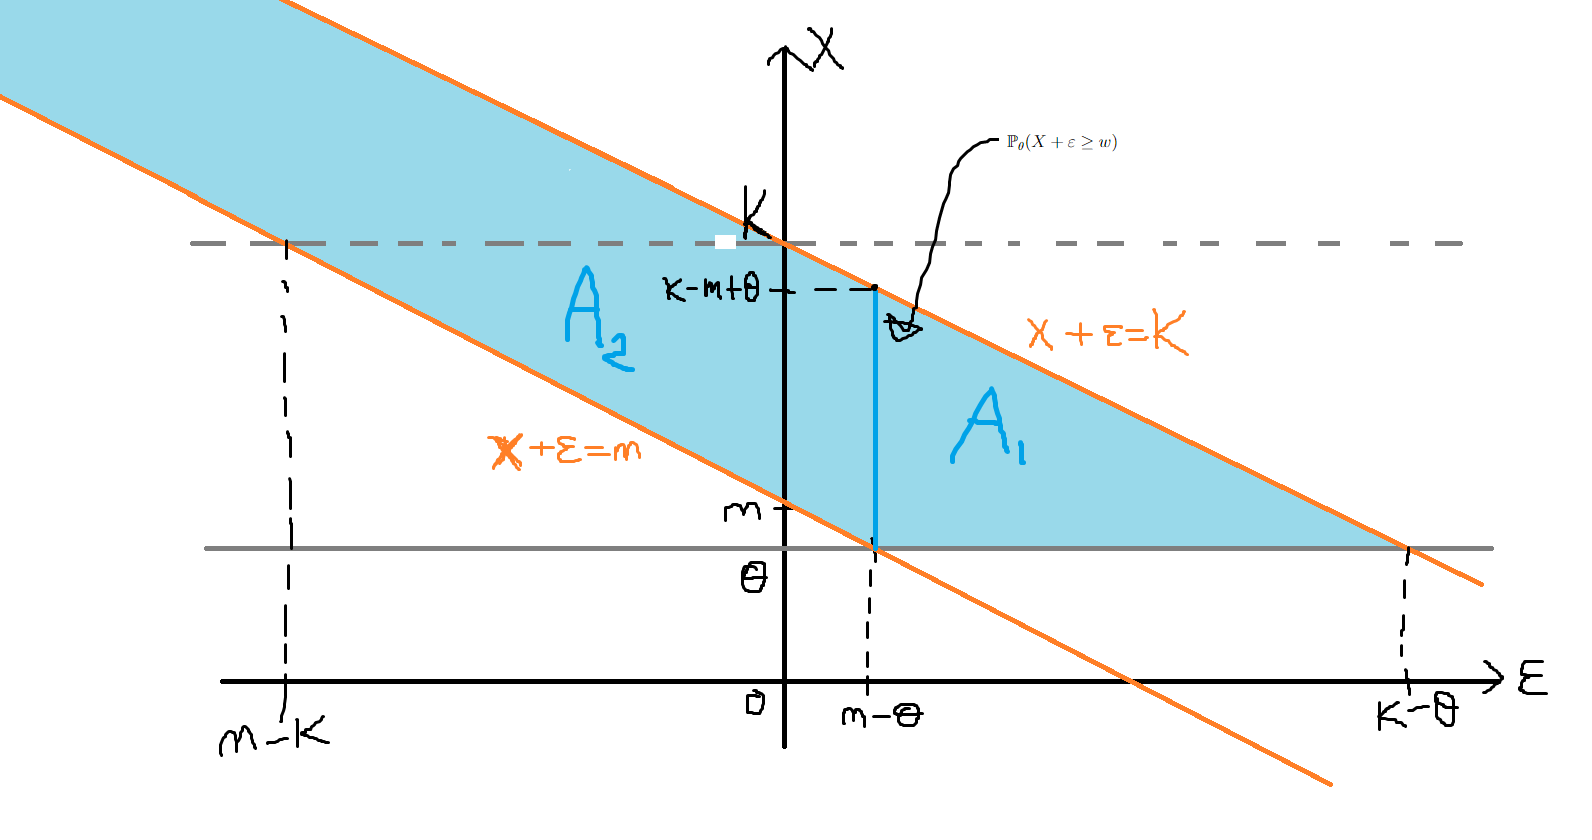
\includegraphics[width=0.8\textwidth]{figures/minmi-integral-sketch.png}
    \caption{Sketch of the region to integrate over}
    \label{fig: minmi_integral}
\end{figure}

Let our statistic $S(\bm{W})$ be the minimum statistic $\min(W_1, \dots, W_n)$, $m = S(\bm{w})$ be the observed minimum, and $\theta_q$ be the $q\textsuperscript{th}$ quantile such that $\PP_{\theta_q} (S(\bm{W}) \geq m) = q$: \begin{align*}
    q &= \PP_{\theta_q} (S(\bm{W}) \geq m) \\
        &= \prod_{i=1}^n \PP_{\theta_q} (X_{i} + \varepsilon_i \geq m) \\
        &= \left[ 1 - \frac{F_\varepsilon(m-\theta_q)}{F_\varepsilon(K - \theta_q)} \psi(\theta_q; m)  \right]^n \\
    q^{\frac{1}{n}} &= 1 - \frac{F_\varepsilon(m-\theta_q)}{F_\varepsilon(K - \theta_q)} \psi(\theta_q; m) \numberthis \label{eqn: minmi-ee}
\end{align*}

The MINMI estimator $\hat\theta_q$ can be found using inversion by solving the above equation for $\theta = \hat\theta_q$. However, since $\psi$ does not simplify in general, we can approximate it with a Monte Carlo integral using $B$ samples, resulting in the below MINMI estimating equation: \begin{align*}
    q^{\frac{1}{n}} &= 1 - \frac{F_\varepsilon(m - \theta_q)}{F_\varepsilon(K - \theta_q)} \hat\psi_B(\theta_q; m); &\hat\psi_B(\theta_q; m) =  \frac{1}{B} \sum_{b=1}^B \frac{m-e_b-\hat\theta_q}{K-e_b-\theta_q} \numberthis \label{eqn: minmi-ee-mc}
\end{align*}

where $e_b$ are drawn from $f_\varepsilon(e_b)$ truncated at $m-\hat\theta_q$

Generating confidence intervals by inversion is conditional on $\PP_{\theta_q} (S(\bm{W}) \geq m)$ being stochastically increasing in $\theta$. This is true under two conditions, shown in \autoref{apx:minmi-stoch-incr-proof}: that $f(e)$ is symmetric and unimodal about 0; and $f(2|m-\theta|) > f(K-\theta) \left(2 + \frac{K-\theta}{|m-\theta|} \right)$, where $f(\cdot)$ denotes the probability density function of $\varepsilon$.

\subsection{Asymptotic Properties}

We now discuss the asymptotic properties of the MINMI estimator. The delta method gives the approximate result \begin{equation}
    \Var(\hat\theta_q) \approx \sigma^2_{\psi(\theta_q)} \left[ \frac{F(K-\theta_q)}{f(K-\theta) \hat\psi(\theta_q) + F(K-\theta) \hat\psi^\prime(\theta_q)} \right]^2
\end{equation}

A full derivation of this result is given in \autoref{apx:minmi-asymptotics-proof}. In general, we do not have know the true value of $\theta_q$ or $\sigma^2_{\psi(\theta_q)}$. Thus, the asymptotic variance must be further approximated by substituting some ``gold standard" estimate of $\theta_q$, $\hat\theta^*_{q}$ (for example, by using a large value of $B$) and using a Monte Carlo estimate of $\sigma^2_{\psi(\theta_q)}$.

We were also able to verify these results by simulation, generating estimates for upper and lower endpoints of a central $95\%$ confidence interval across different values of $B$. These are shown in \autoref{fig:asymptotics-plots} where the blue lines (representing the sample variance of $\hat\theta_q$) and the red lines (representing the variance calculated using the asymptotic approximation formula) converge as $B$ increases. The approximate variance tends to under estimate the variance for small $B$.

\begin{figure}[ht]
    \centering
    \resizebox{0.45\linewidth}{!}{% Created by tikzDevice version 0.12.3.1 on 2022-10-23 12:31:10
% !TEX encoding = UTF-8 Unicode
\begin{tikzpicture}[x=1pt,y=1pt]
\definecolor{fillColor}{RGB}{255,255,255}
\path[use as bounding box,fill=fillColor,fill opacity=0.00] (0,0) rectangle (505.89,505.89);
\begin{scope}
\path[clip] ( 49.20, 61.20) rectangle (480.69,456.69);
\definecolor{drawColor}{RGB}{0,0,255}

\path[draw=drawColor,line width= 0.4pt,line join=round,line cap=round] ( 69.58,437.96) -- ( 81.49,426.88);

\path[draw=drawColor,line width= 0.4pt,line join=round,line cap=round] ( 91.56,420.84) -- ( 94.90,419.69);

\path[draw=drawColor,line width= 0.4pt,line join=round,line cap=round] (104.96,413.63) -- (107.58,411.19);

\path[draw=drawColor,line width= 0.4pt,line join=round,line cap=round] (116.17,402.81) -- (124.95,393.85);

\path[draw=drawColor,line width= 0.4pt,line join=round,line cap=round] (139.92,379.25) -- (143.42,375.25);

\path[draw=drawColor,line width= 0.4pt,line join=round,line cap=round] (152.01,366.93) -- (152.03,366.91);

\path[draw=drawColor,line width= 0.4pt,line join=round,line cap=round] (161.19,359.16) -- (163.55,357.09);

\path[draw=drawColor,line width= 0.4pt,line join=round,line cap=round] (172.06,348.66) -- (173.39,347.15);

\path[draw=drawColor,line width= 0.4pt,line join=round,line cap=round] (181.63,338.43) -- (183.38,336.67);

\path[draw=drawColor,line width= 0.4pt,line join=round,line cap=round] (191.02,327.49) -- (194.69,322.14);

\path[draw=drawColor,line width= 0.4pt,line join=round,line cap=round] (202.76,313.43) -- (203.66,312.71);

\path[draw=drawColor,line width= 0.4pt,line join=round,line cap=round] (213.33,305.63) -- (214.42,304.90);

\path[draw=drawColor,line width= 0.4pt,line join=round,line cap=round] (233.85,292.13) -- (235.40,290.62);

\path[draw=drawColor,line width= 0.4pt,line join=round,line cap=round] (244.33,282.62) -- (244.94,282.11);

\path[draw=drawColor,line width= 0.4pt,line join=round,line cap=round] (253.32,273.61) -- (255.81,270.50);

\path[draw=drawColor,line width= 0.4pt,line join=round,line cap=round] (263.82,261.59) -- (266.02,259.39);

\path[draw=drawColor,line width= 0.4pt,line join=round,line cap=round] (274.72,251.13) -- (275.83,250.12);

\path[draw=drawColor,line width= 0.4pt,line join=round,line cap=round] (284.91,242.28) -- (285.87,241.49);

\path[draw=drawColor,line width= 0.4pt,line join=round,line cap=round] (295.01,233.72) -- (296.35,232.53);

\path[draw=drawColor,line width= 0.4pt,line join=round,line cap=round] (305.35,224.58) -- (306.62,223.47);

\path[draw=drawColor,line width= 0.4pt,line join=round,line cap=round] (314.76,214.73) -- (317.57,211.04);

\path[draw=drawColor,line width= 0.4pt,line join=round,line cap=round] (326.29,203.08) -- (326.40,203.01);

\path[draw=drawColor,line width= 0.4pt,line join=round,line cap=round] (336.18,196.09) -- (337.04,195.41);

\path[draw=drawColor,line width= 0.4pt,line join=round,line cap=round] (346.77,188.41) -- (346.97,188.28);

\path[draw=drawColor,line width= 0.4pt,line join=round,line cap=round] (356.34,180.86) -- (357.96,179.32);

\path[draw=drawColor,line width= 0.4pt,line join=round,line cap=round] (366.55,170.94) -- (368.27,169.21);

\path[draw=drawColor,line width= 0.4pt,line join=round,line cap=round] (377.00,160.98) -- (378.29,159.83);

\path[draw=drawColor,line width= 0.4pt,line join=round,line cap=round] (387.12,151.70) -- (388.67,150.22);

\path[draw=drawColor,line width= 0.4pt,line join=round,line cap=round] (396.54,141.23) -- (399.70,136.90);

\path[draw=drawColor,line width= 0.4pt,line join=round,line cap=round] (407.39,127.73) -- (409.33,125.72);

\path[draw=drawColor,line width= 0.4pt,line join=round,line cap=round] (417.94,117.37) -- (419.28,116.15);

\path[draw=drawColor,line width= 0.4pt,line join=round,line cap=round] (427.77,107.69) -- (429.93,105.32);

\path[draw=drawColor,line width= 0.4pt,line join=round,line cap=round] (438.71, 97.20) -- (439.48, 96.61);

\path[draw=drawColor,line width= 0.4pt,line join=round,line cap=round] (457.99, 85.94) -- (461.18, 81.57);

\path[draw=drawColor,line width= 0.4pt,line join=round,line cap=round] ( 65.18,442.04) circle (  2.25);

\path[draw=drawColor,line width= 0.4pt,line join=round,line cap=round] ( 85.89,422.80) circle (  2.25);

\path[draw=drawColor,line width= 0.4pt,line join=round,line cap=round] (100.58,417.73) circle (  2.25);

\path[draw=drawColor,line width= 0.4pt,line join=round,line cap=round] (111.97,407.10) circle (  2.25);

\path[draw=drawColor,line width= 0.4pt,line join=round,line cap=round] (129.15,389.57) circle (  2.25);

\path[draw=drawColor,line width= 0.4pt,line join=round,line cap=round] (135.97,383.77) circle (  2.25);

\path[draw=drawColor,line width= 0.4pt,line join=round,line cap=round] (147.37,370.73) circle (  2.25);

\path[draw=drawColor,line width= 0.4pt,line join=round,line cap=round] (156.68,363.11) circle (  2.25);

\path[draw=drawColor,line width= 0.4pt,line join=round,line cap=round] (168.07,353.14) circle (  2.25);

\path[draw=drawColor,line width= 0.4pt,line join=round,line cap=round] (177.38,342.67) circle (  2.25);

\path[draw=drawColor,line width= 0.4pt,line join=round,line cap=round] (187.63,332.43) circle (  2.25);

\path[draw=drawColor,line width= 0.4pt,line join=round,line cap=round] (198.09,317.19) circle (  2.25);

\path[draw=drawColor,line width= 0.4pt,line join=round,line cap=round] (208.33,308.95) circle (  2.25);

\path[draw=drawColor,line width= 0.4pt,line join=round,line cap=round] (219.42,301.57) circle (  2.25);

\path[draw=drawColor,line width= 0.4pt,line join=round,line cap=round] (229.55,296.32) circle (  2.25);

\path[draw=drawColor,line width= 0.4pt,line join=round,line cap=round] (239.70,286.44) circle (  2.25);

\path[draw=drawColor,line width= 0.4pt,line join=round,line cap=round] (249.57,278.29) circle (  2.25);

\path[draw=drawColor,line width= 0.4pt,line join=round,line cap=round] (259.56,265.82) circle (  2.25);

\path[draw=drawColor,line width= 0.4pt,line join=round,line cap=round] (270.27,255.16) circle (  2.25);

\path[draw=drawColor,line width= 0.4pt,line join=round,line cap=round] (280.27,246.08) circle (  2.25);

\path[draw=drawColor,line width= 0.4pt,line join=round,line cap=round] (290.52,237.69) circle (  2.25);

\path[draw=drawColor,line width= 0.4pt,line join=round,line cap=round] (300.85,228.55) circle (  2.25);

\path[draw=drawColor,line width= 0.4pt,line join=round,line cap=round] (311.12,219.50) circle (  2.25);

\path[draw=drawColor,line width= 0.4pt,line join=round,line cap=round] (321.21,206.27) circle (  2.25);

\path[draw=drawColor,line width= 0.4pt,line join=round,line cap=round] (331.48,199.82) circle (  2.25);

\path[draw=drawColor,line width= 0.4pt,line join=round,line cap=round] (341.75,191.68) circle (  2.25);

\path[draw=drawColor,line width= 0.4pt,line join=round,line cap=round] (352.00,185.00) circle (  2.25);

\path[draw=drawColor,line width= 0.4pt,line join=round,line cap=round] (362.30,175.18) circle (  2.25);

\path[draw=drawColor,line width= 0.4pt,line join=round,line cap=round] (372.52,164.97) circle (  2.25);

\path[draw=drawColor,line width= 0.4pt,line join=round,line cap=round] (382.78,155.85) circle (  2.25);

\path[draw=drawColor,line width= 0.4pt,line join=round,line cap=round] (393.01,146.08) circle (  2.25);

\path[draw=drawColor,line width= 0.4pt,line join=round,line cap=round] (403.23,132.05) circle (  2.25);

\path[draw=drawColor,line width= 0.4pt,line join=round,line cap=round] (413.49,121.40) circle (  2.25);

\path[draw=drawColor,line width= 0.4pt,line join=round,line cap=round] (423.73,112.12) circle (  2.25);

\path[draw=drawColor,line width= 0.4pt,line join=round,line cap=round] (433.98,100.88) circle (  2.25);

\path[draw=drawColor,line width= 0.4pt,line join=round,line cap=round] (444.21, 92.93) circle (  2.25);

\path[draw=drawColor,line width= 0.4pt,line join=round,line cap=round] (454.46, 90.79) circle (  2.25);

\path[draw=drawColor,line width= 0.4pt,line join=round,line cap=round] (464.71, 76.72) circle (  2.25);
\end{scope}
\begin{scope}
\path[clip] (  0.00,  0.00) rectangle (505.89,505.89);
\definecolor{drawColor}{RGB}{0,0,0}

\path[draw=drawColor,line width= 0.4pt,line join=round,line cap=round] ( 65.18, 61.20) -- (464.71, 61.20);

\path[draw=drawColor,line width= 0.4pt,line join=round,line cap=round] ( 65.18, 61.20) -- ( 65.18, 55.20);

\path[draw=drawColor,line width= 0.4pt,line join=round,line cap=round] (111.97, 61.20) -- (111.97, 55.20);

\path[draw=drawColor,line width= 0.4pt,line join=round,line cap=round] (147.37, 61.20) -- (147.37, 55.20);

\path[draw=drawColor,line width= 0.4pt,line join=round,line cap=round] (182.76, 61.20) -- (182.76, 55.20);

\path[draw=drawColor,line width= 0.4pt,line join=round,line cap=round] (229.55, 61.20) -- (229.55, 55.20);

\path[draw=drawColor,line width= 0.4pt,line join=round,line cap=round] (264.94, 61.20) -- (264.94, 55.20);

\path[draw=drawColor,line width= 0.4pt,line join=round,line cap=round] (300.34, 61.20) -- (300.34, 55.20);

\path[draw=drawColor,line width= 0.4pt,line join=round,line cap=round] (347.13, 61.20) -- (347.13, 55.20);

\path[draw=drawColor,line width= 0.4pt,line join=round,line cap=round] (382.52, 61.20) -- (382.52, 55.20);

\path[draw=drawColor,line width= 0.4pt,line join=round,line cap=round] (417.92, 61.20) -- (417.92, 55.20);

\path[draw=drawColor,line width= 0.4pt,line join=round,line cap=round] (464.71, 61.20) -- (464.71, 55.20);

\node[text=drawColor,anchor=base,inner sep=0pt, outer sep=0pt, scale=  1.00] at ( 65.18, 39.60) {2};

\node[text=drawColor,anchor=base,inner sep=0pt, outer sep=0pt, scale=  1.00] at (111.97, 39.60) {5};

\node[text=drawColor,anchor=base,inner sep=0pt, outer sep=0pt, scale=  1.00] at (147.37, 39.60) {10};

\node[text=drawColor,anchor=base,inner sep=0pt, outer sep=0pt, scale=  1.00] at (182.76, 39.60) {20};

\node[text=drawColor,anchor=base,inner sep=0pt, outer sep=0pt, scale=  1.00] at (229.55, 39.60) {50};

\node[text=drawColor,anchor=base,inner sep=0pt, outer sep=0pt, scale=  1.00] at (264.94, 39.60) {100};

\node[text=drawColor,anchor=base,inner sep=0pt, outer sep=0pt, scale=  1.00] at (300.34, 39.60) {200};

\node[text=drawColor,anchor=base,inner sep=0pt, outer sep=0pt, scale=  1.00] at (347.13, 39.60) {500};

\node[text=drawColor,anchor=base,inner sep=0pt, outer sep=0pt, scale=  1.00] at (382.52, 39.60) {1000};

\node[text=drawColor,anchor=base,inner sep=0pt, outer sep=0pt, scale=  1.00] at (417.92, 39.60) {2000};

\node[text=drawColor,anchor=base,inner sep=0pt, outer sep=0pt, scale=  1.00] at (464.71, 39.60) {5000};

\path[draw=drawColor,line width= 0.4pt,line join=round,line cap=round] ( 49.20, 90.55) -- ( 49.20,415.62);

\path[draw=drawColor,line width= 0.4pt,line join=round,line cap=round] ( 49.20, 90.55) -- ( 43.20, 90.55);

\path[draw=drawColor,line width= 0.4pt,line join=round,line cap=round] ( 49.20,133.67) -- ( 43.20,133.67);

\path[draw=drawColor,line width= 0.4pt,line join=round,line cap=round] ( 49.20,166.29) -- ( 43.20,166.29);

\path[draw=drawColor,line width= 0.4pt,line join=round,line cap=round] ( 49.20,198.91) -- ( 43.20,198.91);

\path[draw=drawColor,line width= 0.4pt,line join=round,line cap=round] ( 49.20,242.03) -- ( 43.20,242.03);

\path[draw=drawColor,line width= 0.4pt,line join=round,line cap=round] ( 49.20,274.64) -- ( 43.20,274.64);

\path[draw=drawColor,line width= 0.4pt,line join=round,line cap=round] ( 49.20,307.26) -- ( 43.20,307.26);

\path[draw=drawColor,line width= 0.4pt,line join=round,line cap=round] ( 49.20,350.38) -- ( 43.20,350.38);

\path[draw=drawColor,line width= 0.4pt,line join=round,line cap=round] ( 49.20,383.00) -- ( 43.20,383.00);

\path[draw=drawColor,line width= 0.4pt,line join=round,line cap=round] ( 49.20,415.62) -- ( 43.20,415.62);

\node[text=drawColor,rotate= 90.00,anchor=base,inner sep=0pt, outer sep=0pt, scale=  1.00] at ( 34.80, 90.55) {20};

\node[text=drawColor,rotate= 90.00,anchor=base,inner sep=0pt, outer sep=0pt, scale=  1.00] at ( 34.80,133.67) {50};

\node[text=drawColor,rotate= 90.00,anchor=base,inner sep=0pt, outer sep=0pt, scale=  1.00] at ( 34.80,166.29) {100};

\node[text=drawColor,rotate= 90.00,anchor=base,inner sep=0pt, outer sep=0pt, scale=  1.00] at ( 34.80,198.91) {200};

\node[text=drawColor,rotate= 90.00,anchor=base,inner sep=0pt, outer sep=0pt, scale=  1.00] at ( 34.80,242.03) {500};

\node[text=drawColor,rotate= 90.00,anchor=base,inner sep=0pt, outer sep=0pt, scale=  1.00] at ( 34.80,274.64) {1000};

\node[text=drawColor,rotate= 90.00,anchor=base,inner sep=0pt, outer sep=0pt, scale=  1.00] at ( 34.80,307.26) {2000};

\node[text=drawColor,rotate= 90.00,anchor=base,inner sep=0pt, outer sep=0pt, scale=  1.00] at ( 34.80,350.38) {5000};

\node[text=drawColor,rotate= 90.00,anchor=base,inner sep=0pt, outer sep=0pt, scale=  1.00] at ( 34.80,383.00) {10000};

\path[draw=drawColor,line width= 0.4pt,line join=round,line cap=round] ( 49.20, 61.20) --
	(480.69, 61.20) --
	(480.69,456.69) --
	( 49.20,456.69) --
	cycle;
\end{scope}
\begin{scope}
\path[clip] (  0.00,  0.00) rectangle (505.89,505.89);
\definecolor{drawColor}{RGB}{0,0,0}

\node[text=drawColor,anchor=base,inner sep=0pt, outer sep=0pt, scale=  1.20] at (264.94,477.15) {\bfseries Sample Var vs. Delta Method (q=0.025)};

\node[text=drawColor,anchor=base,inner sep=0pt, outer sep=0pt, scale=  1.00] at (264.94, 15.60) {B};
\end{scope}
\begin{scope}
\path[clip] ( 49.20, 61.20) rectangle (480.69,456.69);
\definecolor{drawColor}{RGB}{255,0,0}

\path[draw=drawColor,line width= 0.4pt,line join=round,line cap=round] ( 69.51,412.63) -- ( 81.56,401.07);

\path[draw=drawColor,line width= 0.4pt,line join=round,line cap=round] ( 88.36,391.45) -- ( 98.11,369.86);

\path[draw=drawColor,line width= 0.4pt,line join=round,line cap=round] (114.52,366.36) -- (126.60,392.05);

\path[draw=drawColor,line width= 0.4pt,line join=round,line cap=round] (132.50,392.50) -- (132.62,392.33);

\path[draw=drawColor,line width= 0.4pt,line join=round,line cap=round] (139.06,382.20) -- (144.28,373.52);

\path[draw=drawColor,line width= 0.4pt,line join=round,line cap=round] (160.50,358.36) -- (164.25,353.82);

\path[draw=drawColor,line width= 0.4pt,line join=round,line cap=round] (171.21,344.08) -- (174.24,339.16);

\path[draw=drawColor,line width= 0.4pt,line join=round,line cap=round] (180.51,328.93) -- (184.50,322.42);

\path[draw=drawColor,line width= 0.4pt,line join=round,line cap=round] (202.57,314.00) -- (203.85,312.86);

\path[draw=drawColor,line width= 0.4pt,line join=round,line cap=round] (211.77,303.96) -- (215.97,297.97);

\path[draw=drawColor,line width= 0.4pt,line join=round,line cap=round] (223.75,288.90) -- (225.22,287.48);

\path[draw=drawColor,line width= 0.4pt,line join=round,line cap=round] (234.16,279.49) -- (235.10,278.70);

\path[draw=drawColor,line width= 0.4pt,line join=round,line cap=round] (243.71,270.39) -- (245.56,268.32);

\path[draw=drawColor,line width= 0.4pt,line join=round,line cap=round] (264.71,256.55) -- (265.13,256.29);

\path[draw=drawColor,line width= 0.4pt,line join=round,line cap=round] (273.94,248.45) -- (276.60,245.01);

\path[draw=drawColor,line width= 0.4pt,line join=round,line cap=round] (295.43,230.67) -- (295.94,230.31);

\path[draw=drawColor,line width= 0.4pt,line join=round,line cap=round] (305.43,223.00) -- (306.53,222.06);

\path[draw=drawColor,line width= 0.4pt,line join=round,line cap=round] (315.82,214.46) -- (316.52,213.90);

\path[draw=drawColor,line width= 0.4pt,line join=round,line cap=round] (325.40,205.87) -- (327.30,203.91);

\path[draw=drawColor,line width= 0.4pt,line join=round,line cap=round] (335.89,195.54) -- (337.34,194.21);

\path[draw=drawColor,line width= 0.4pt,line join=round,line cap=round] (345.64,185.58) -- (348.10,182.70);

\path[draw=drawColor,line width= 0.4pt,line join=round,line cap=round] (356.21,173.86) -- (358.09,171.95);

\path[draw=drawColor,line width= 0.4pt,line join=round,line cap=round] (366.81,163.71) -- (368.01,162.66);

\path[draw=drawColor,line width= 0.4pt,line join=round,line cap=round] (376.97,154.69) -- (378.32,153.48);

\path[draw=drawColor,line width= 0.4pt,line join=round,line cap=round] (387.38,145.62) -- (388.41,144.75);

\path[draw=drawColor,line width= 0.4pt,line join=round,line cap=round] (397.38,136.79) -- (398.86,135.40);

\path[draw=drawColor,line width= 0.4pt,line join=round,line cap=round] (407.80,127.40) -- (408.93,126.43);

\path[draw=drawColor,line width= 0.4pt,line join=round,line cap=round] (417.93,118.50) -- (419.29,117.26);

\path[draw=drawColor,line width= 0.4pt,line join=round,line cap=round] (428.18,109.20) -- (429.52,107.99);

\path[draw=drawColor,line width= 0.4pt,line join=round,line cap=round] (438.51,100.04) -- (439.68, 99.02);

\path[draw=drawColor,line width= 0.4pt,line join=round,line cap=round] (448.43, 90.82) -- (450.25, 88.98);

\path[draw=drawColor,line width= 0.4pt,line join=round,line cap=round] (459.00, 80.78) -- (460.17, 79.77);

\path[draw=drawColor,line width= 0.4pt,line join=round,line cap=round] ( 65.18,416.78) circle (  2.25);

\path[draw=drawColor,line width= 0.4pt,line join=round,line cap=round] ( 85.89,396.92) circle (  2.25);

\path[draw=drawColor,line width= 0.4pt,line join=round,line cap=round] (100.58,364.39) circle (  2.25);

\path[draw=drawColor,line width= 0.4pt,line join=round,line cap=round] (111.97,360.93) circle (  2.25);

\path[draw=drawColor,line width= 0.4pt,line join=round,line cap=round] (129.15,397.48) circle (  2.25);

\path[draw=drawColor,line width= 0.4pt,line join=round,line cap=round] (135.97,387.35) circle (  2.25);

\path[draw=drawColor,line width= 0.4pt,line join=round,line cap=round] (147.37,368.37) circle (  2.25);

\path[draw=drawColor,line width= 0.4pt,line join=round,line cap=round] (156.68,362.98) circle (  2.25);

\path[draw=drawColor,line width= 0.4pt,line join=round,line cap=round] (168.07,349.20) circle (  2.25);

\path[draw=drawColor,line width= 0.4pt,line join=round,line cap=round] (177.38,334.05) circle (  2.25);

\path[draw=drawColor,line width= 0.4pt,line join=round,line cap=round] (187.63,317.30) circle (  2.25);

\path[draw=drawColor,line width= 0.4pt,line join=round,line cap=round] (198.09,317.98) circle (  2.25);

\path[draw=drawColor,line width= 0.4pt,line join=round,line cap=round] (208.33,308.88) circle (  2.25);

\path[draw=drawColor,line width= 0.4pt,line join=round,line cap=round] (219.42,293.05) circle (  2.25);

\path[draw=drawColor,line width= 0.4pt,line join=round,line cap=round] (229.55,283.33) circle (  2.25);

\path[draw=drawColor,line width= 0.4pt,line join=round,line cap=round] (239.70,274.86) circle (  2.25);

\path[draw=drawColor,line width= 0.4pt,line join=round,line cap=round] (249.57,263.85) circle (  2.25);

\path[draw=drawColor,line width= 0.4pt,line join=round,line cap=round] (259.56,259.65) circle (  2.25);

\path[draw=drawColor,line width= 0.4pt,line join=round,line cap=round] (270.27,253.20) circle (  2.25);

\path[draw=drawColor,line width= 0.4pt,line join=round,line cap=round] (280.27,240.26) circle (  2.25);

\path[draw=drawColor,line width= 0.4pt,line join=round,line cap=round] (290.52,234.11) circle (  2.25);

\path[draw=drawColor,line width= 0.4pt,line join=round,line cap=round] (300.85,226.87) circle (  2.25);

\path[draw=drawColor,line width= 0.4pt,line join=round,line cap=round] (311.12,218.19) circle (  2.25);

\path[draw=drawColor,line width= 0.4pt,line join=round,line cap=round] (321.21,210.17) circle (  2.25);

\path[draw=drawColor,line width= 0.4pt,line join=round,line cap=round] (331.48,199.61) circle (  2.25);

\path[draw=drawColor,line width= 0.4pt,line join=round,line cap=round] (341.75,190.15) circle (  2.25);

\path[draw=drawColor,line width= 0.4pt,line join=round,line cap=round] (352.00,178.14) circle (  2.25);

\path[draw=drawColor,line width= 0.4pt,line join=round,line cap=round] (362.30,167.67) circle (  2.25);

\path[draw=drawColor,line width= 0.4pt,line join=round,line cap=round] (372.52,158.70) circle (  2.25);

\path[draw=drawColor,line width= 0.4pt,line join=round,line cap=round] (382.78,149.47) circle (  2.25);

\path[draw=drawColor,line width= 0.4pt,line join=round,line cap=round] (393.01,140.91) circle (  2.25);

\path[draw=drawColor,line width= 0.4pt,line join=round,line cap=round] (403.23,131.29) circle (  2.25);

\path[draw=drawColor,line width= 0.4pt,line join=round,line cap=round] (413.49,122.54) circle (  2.25);

\path[draw=drawColor,line width= 0.4pt,line join=round,line cap=round] (423.73,113.22) circle (  2.25);

\path[draw=drawColor,line width= 0.4pt,line join=round,line cap=round] (433.98,103.97) circle (  2.25);

\path[draw=drawColor,line width= 0.4pt,line join=round,line cap=round] (444.21, 95.09) circle (  2.25);

\path[draw=drawColor,line width= 0.4pt,line join=round,line cap=round] (454.46, 84.70) circle (  2.25);

\path[draw=drawColor,line width= 0.4pt,line join=round,line cap=round] (464.71, 75.85) circle (  2.25);
\definecolor{drawColor}{RGB}{0,0,0}

\path[draw=drawColor,line width= 0.4pt,line join=round,line cap=round] (395.89,456.69) rectangle (480.69,420.69);
\definecolor{drawColor}{RGB}{0,0,255}

\path[draw=drawColor,line width= 0.4pt,line join=round,line cap=round] (398.59,444.69) -- (416.59,444.69);
\definecolor{drawColor}{RGB}{255,0,0}

\path[draw=drawColor,line width= 0.4pt,line join=round,line cap=round] (398.59,432.69) -- (416.59,432.69);
\definecolor{drawColor}{RGB}{0,0,255}

\path[draw=drawColor,line width= 0.4pt,line join=round,line cap=round] (407.59,444.69) circle (  2.25);
\definecolor{drawColor}{RGB}{255,0,0}

\path[draw=drawColor,line width= 0.4pt,line join=round,line cap=round] (407.59,432.69) circle (  2.25);
\definecolor{drawColor}{RGB}{0,0,0}

\node[text=drawColor,anchor=base west,inner sep=0pt, outer sep=0pt, scale=  1.00] at (425.59,441.25) {Sample Var};

\node[text=drawColor,anchor=base west,inner sep=0pt, outer sep=0pt, scale=  1.00] at (425.59,429.25) {Asymptotic};
\end{scope}
\end{tikzpicture}
}
    \resizebox{0.45\linewidth}{!}{% Created by tikzDevice version 0.12.3.1 on 2022-10-23 12:41:59
% !TEX encoding = UTF-8 Unicode
\begin{tikzpicture}[x=1pt,y=1pt]
\definecolor{fillColor}{RGB}{255,255,255}
\path[use as bounding box,fill=fillColor,fill opacity=0.00] (0,0) rectangle (505.89,505.89);
\begin{scope}
\path[clip] ( 49.20, 61.20) rectangle (480.69,456.69);
\definecolor{drawColor}{RGB}{0,0,255}

\path[draw=drawColor,line width= 0.4pt,line join=round,line cap=round] ( 69.28,437.66) -- ( 81.79,424.26);

\path[draw=drawColor,line width= 0.4pt,line join=round,line cap=round] ( 91.30,417.28) -- ( 95.16,415.43);

\path[draw=drawColor,line width= 0.4pt,line join=round,line cap=round] (105.05,408.85) -- (107.49,406.67);

\path[draw=drawColor,line width= 0.4pt,line join=round,line cap=round] (115.92,398.16) -- (125.20,387.54);

\path[draw=drawColor,line width= 0.4pt,line join=round,line cap=round] (139.79,374.08) -- (143.55,369.53);

\path[draw=drawColor,line width= 0.4pt,line join=round,line cap=round] (161.20,353.80) -- (163.54,351.77);

\path[draw=drawColor,line width= 0.4pt,line join=round,line cap=round] (172.10,343.39) -- (173.35,342.02);

\path[draw=drawColor,line width= 0.4pt,line join=round,line cap=round] (181.30,333.04) -- (183.71,330.25);

\path[draw=drawColor,line width= 0.4pt,line join=round,line cap=round] (191.31,320.97) -- (194.40,317.00);

\path[draw=drawColor,line width= 0.4pt,line join=round,line cap=round] (202.00,307.72) -- (204.42,304.92);

\path[draw=drawColor,line width= 0.4pt,line join=round,line cap=round] (213.44,297.22) -- (214.31,296.67);

\path[draw=drawColor,line width= 0.4pt,line join=round,line cap=round] (233.73,284.16) -- (235.53,282.31);

\path[draw=drawColor,line width= 0.4pt,line join=round,line cap=round] (244.10,273.91) -- (245.18,272.91);

\path[draw=drawColor,line width= 0.4pt,line join=round,line cap=round] (253.21,264.05) -- (255.92,260.50);

\path[draw=drawColor,line width= 0.4pt,line join=round,line cap=round] (263.51,251.22) -- (266.33,247.98);

\path[draw=drawColor,line width= 0.4pt,line join=round,line cap=round] (275.20,240.04) -- (275.34,239.94);

\path[draw=drawColor,line width= 0.4pt,line join=round,line cap=round] (285.07,232.92) -- (285.72,232.43);

\path[draw=drawColor,line width= 0.4pt,line join=round,line cap=round] (294.97,224.81) -- (296.39,223.53);

\path[draw=drawColor,line width= 0.4pt,line join=round,line cap=round] (305.42,215.63) -- (306.54,214.67);

\path[draw=drawColor,line width= 0.4pt,line join=round,line cap=round] (315.00,206.21) -- (317.33,203.47);

\path[draw=drawColor,line width= 0.4pt,line join=round,line cap=round] (336.55,191.02) -- (336.68,190.94);

\path[draw=drawColor,line width= 0.4pt,line join=round,line cap=round] (356.38,179.11) -- (357.92,177.68);

\path[draw=drawColor,line width= 0.4pt,line join=round,line cap=round] (366.95,169.80) -- (367.86,169.06);

\path[draw=drawColor,line width= 0.4pt,line join=round,line cap=round] (377.31,161.67) -- (377.98,161.17);

\path[draw=drawColor,line width= 0.4pt,line join=round,line cap=round] (387.19,153.50) -- (388.60,152.21);

\path[draw=drawColor,line width= 0.4pt,line join=round,line cap=round] (396.67,143.39) -- (399.57,139.62);

\path[draw=drawColor,line width= 0.4pt,line join=round,line cap=round] (407.43,130.58) -- (409.29,128.68);

\path[draw=drawColor,line width= 0.4pt,line join=round,line cap=round] (417.71,120.13) -- (419.51,118.30);

\path[draw=drawColor,line width= 0.4pt,line join=round,line cap=round] (427.84,109.66) -- (429.87,107.50);

\path[draw=drawColor,line width= 0.4pt,line join=round,line cap=round] (438.52, 99.22) -- (439.67, 98.24);

\path[draw=drawColor,line width= 0.4pt,line join=round,line cap=round] (458.75, 86.61) -- (460.43, 84.96);

\path[draw=drawColor,line width= 0.4pt,line join=round,line cap=round] ( 65.18,442.04) circle (  2.25);

\path[draw=drawColor,line width= 0.4pt,line join=round,line cap=round] ( 85.89,419.88) circle (  2.25);

\path[draw=drawColor,line width= 0.4pt,line join=round,line cap=round] (100.58,412.84) circle (  2.25);

\path[draw=drawColor,line width= 0.4pt,line join=round,line cap=round] (111.97,402.68) circle (  2.25);

\path[draw=drawColor,line width= 0.4pt,line join=round,line cap=round] (129.15,383.02) circle (  2.25);

\path[draw=drawColor,line width= 0.4pt,line join=round,line cap=round] (135.97,378.71) circle (  2.25);

\path[draw=drawColor,line width= 0.4pt,line join=round,line cap=round] (147.37,364.90) circle (  2.25);

\path[draw=drawColor,line width= 0.4pt,line join=round,line cap=round] (156.68,357.74) circle (  2.25);

\path[draw=drawColor,line width= 0.4pt,line join=round,line cap=round] (168.07,347.83) circle (  2.25);

\path[draw=drawColor,line width= 0.4pt,line join=round,line cap=round] (177.38,337.58) circle (  2.25);

\path[draw=drawColor,line width= 0.4pt,line join=round,line cap=round] (187.63,325.71) circle (  2.25);

\path[draw=drawColor,line width= 0.4pt,line join=round,line cap=round] (198.09,312.27) circle (  2.25);

\path[draw=drawColor,line width= 0.4pt,line join=round,line cap=round] (208.33,300.37) circle (  2.25);

\path[draw=drawColor,line width= 0.4pt,line join=round,line cap=round] (219.42,293.52) circle (  2.25);

\path[draw=drawColor,line width= 0.4pt,line join=round,line cap=round] (229.55,288.47) circle (  2.25);

\path[draw=drawColor,line width= 0.4pt,line join=round,line cap=round] (239.70,278.00) circle (  2.25);

\path[draw=drawColor,line width= 0.4pt,line join=round,line cap=round] (249.57,268.82) circle (  2.25);

\path[draw=drawColor,line width= 0.4pt,line join=round,line cap=round] (259.56,255.74) circle (  2.25);

\path[draw=drawColor,line width= 0.4pt,line join=round,line cap=round] (270.27,243.46) circle (  2.25);

\path[draw=drawColor,line width= 0.4pt,line join=round,line cap=round] (280.27,236.52) circle (  2.25);

\path[draw=drawColor,line width= 0.4pt,line join=round,line cap=round] (290.52,228.83) circle (  2.25);

\path[draw=drawColor,line width= 0.4pt,line join=round,line cap=round] (300.85,219.51) circle (  2.25);

\path[draw=drawColor,line width= 0.4pt,line join=round,line cap=round] (311.12,210.79) circle (  2.25);

\path[draw=drawColor,line width= 0.4pt,line join=round,line cap=round] (321.21,198.90) circle (  2.25);

\path[draw=drawColor,line width= 0.4pt,line join=round,line cap=round] (331.48,194.23) circle (  2.25);

\path[draw=drawColor,line width= 0.4pt,line join=round,line cap=round] (341.75,187.73) circle (  2.25);

\path[draw=drawColor,line width= 0.4pt,line join=round,line cap=round] (352.00,183.21) circle (  2.25);

\path[draw=drawColor,line width= 0.4pt,line join=round,line cap=round] (362.30,173.59) circle (  2.25);

\path[draw=drawColor,line width= 0.4pt,line join=round,line cap=round] (372.52,165.27) circle (  2.25);

\path[draw=drawColor,line width= 0.4pt,line join=round,line cap=round] (382.78,157.56) circle (  2.25);

\path[draw=drawColor,line width= 0.4pt,line join=round,line cap=round] (393.01,148.15) circle (  2.25);

\path[draw=drawColor,line width= 0.4pt,line join=round,line cap=round] (403.23,134.86) circle (  2.25);

\path[draw=drawColor,line width= 0.4pt,line join=round,line cap=round] (413.49,124.40) circle (  2.25);

\path[draw=drawColor,line width= 0.4pt,line join=round,line cap=round] (423.73,114.03) circle (  2.25);

\path[draw=drawColor,line width= 0.4pt,line join=round,line cap=round] (433.98,103.13) circle (  2.25);

\path[draw=drawColor,line width= 0.4pt,line join=round,line cap=round] (444.21, 94.32) circle (  2.25);

\path[draw=drawColor,line width= 0.4pt,line join=round,line cap=round] (454.46, 90.81) circle (  2.25);

\path[draw=drawColor,line width= 0.4pt,line join=round,line cap=round] (464.71, 80.76) circle (  2.25);
\end{scope}
\begin{scope}
\path[clip] (  0.00,  0.00) rectangle (505.89,505.89);
\definecolor{drawColor}{RGB}{0,0,0}

\path[draw=drawColor,line width= 0.4pt,line join=round,line cap=round] ( 65.18, 61.20) -- (464.71, 61.20);

\path[draw=drawColor,line width= 0.4pt,line join=round,line cap=round] ( 65.18, 61.20) -- ( 65.18, 55.20);

\path[draw=drawColor,line width= 0.4pt,line join=round,line cap=round] (111.97, 61.20) -- (111.97, 55.20);

\path[draw=drawColor,line width= 0.4pt,line join=round,line cap=round] (147.37, 61.20) -- (147.37, 55.20);

\path[draw=drawColor,line width= 0.4pt,line join=round,line cap=round] (182.76, 61.20) -- (182.76, 55.20);

\path[draw=drawColor,line width= 0.4pt,line join=round,line cap=round] (229.55, 61.20) -- (229.55, 55.20);

\path[draw=drawColor,line width= 0.4pt,line join=round,line cap=round] (264.94, 61.20) -- (264.94, 55.20);

\path[draw=drawColor,line width= 0.4pt,line join=round,line cap=round] (300.34, 61.20) -- (300.34, 55.20);

\path[draw=drawColor,line width= 0.4pt,line join=round,line cap=round] (347.13, 61.20) -- (347.13, 55.20);

\path[draw=drawColor,line width= 0.4pt,line join=round,line cap=round] (382.52, 61.20) -- (382.52, 55.20);

\path[draw=drawColor,line width= 0.4pt,line join=round,line cap=round] (417.92, 61.20) -- (417.92, 55.20);

\path[draw=drawColor,line width= 0.4pt,line join=round,line cap=round] (464.71, 61.20) -- (464.71, 55.20);

\node[text=drawColor,anchor=base,inner sep=0pt, outer sep=0pt, scale=  1.00] at ( 65.18, 39.60) {2};

\node[text=drawColor,anchor=base,inner sep=0pt, outer sep=0pt, scale=  1.00] at (111.97, 39.60) {5};

\node[text=drawColor,anchor=base,inner sep=0pt, outer sep=0pt, scale=  1.00] at (147.37, 39.60) {10};

\node[text=drawColor,anchor=base,inner sep=0pt, outer sep=0pt, scale=  1.00] at (182.76, 39.60) {20};

\node[text=drawColor,anchor=base,inner sep=0pt, outer sep=0pt, scale=  1.00] at (229.55, 39.60) {50};

\node[text=drawColor,anchor=base,inner sep=0pt, outer sep=0pt, scale=  1.00] at (264.94, 39.60) {100};

\node[text=drawColor,anchor=base,inner sep=0pt, outer sep=0pt, scale=  1.00] at (300.34, 39.60) {200};

\node[text=drawColor,anchor=base,inner sep=0pt, outer sep=0pt, scale=  1.00] at (347.13, 39.60) {500};

\node[text=drawColor,anchor=base,inner sep=0pt, outer sep=0pt, scale=  1.00] at (382.52, 39.60) {1000};

\node[text=drawColor,anchor=base,inner sep=0pt, outer sep=0pt, scale=  1.00] at (417.92, 39.60) {2000};

\node[text=drawColor,anchor=base,inner sep=0pt, outer sep=0pt, scale=  1.00] at (464.71, 39.60) {5000};

\path[draw=drawColor,line width= 0.4pt,line join=round,line cap=round] ( 49.20,114.19) -- ( 49.20,455.01);

\path[draw=drawColor,line width= 0.4pt,line join=round,line cap=round] ( 49.20,114.19) -- ( 43.20,114.19);

\path[draw=drawColor,line width= 0.4pt,line join=round,line cap=round] ( 49.20,145.27) -- ( 43.20,145.27);

\path[draw=drawColor,line width= 0.4pt,line join=round,line cap=round] ( 49.20,217.44) -- ( 43.20,217.44);

\path[draw=drawColor,line width= 0.4pt,line join=round,line cap=round] ( 49.20,248.52) -- ( 43.20,248.52);

\path[draw=drawColor,line width= 0.4pt,line join=round,line cap=round] ( 49.20,320.69) -- ( 43.20,320.69);

\path[draw=drawColor,line width= 0.4pt,line join=round,line cap=round] ( 49.20,351.77) -- ( 43.20,351.77);

\path[draw=drawColor,line width= 0.4pt,line join=round,line cap=round] ( 49.20,423.93) -- ( 43.20,423.93);

\path[draw=drawColor,line width= 0.4pt,line join=round,line cap=round] ( 49.20,455.01) -- ( 43.20,455.01);

\node[text=drawColor,rotate= 90.00,anchor=base,inner sep=0pt, outer sep=0pt, scale=  1.00] at ( 34.80,114.19) {5};

\node[text=drawColor,rotate= 90.00,anchor=base,inner sep=0pt, outer sep=0pt, scale=  1.00] at ( 34.80,145.27) {10};

\node[text=drawColor,rotate= 90.00,anchor=base,inner sep=0pt, outer sep=0pt, scale=  1.00] at ( 34.80,217.44) {50};

\node[text=drawColor,rotate= 90.00,anchor=base,inner sep=0pt, outer sep=0pt, scale=  1.00] at ( 34.80,248.52) {100};

\node[text=drawColor,rotate= 90.00,anchor=base,inner sep=0pt, outer sep=0pt, scale=  1.00] at ( 34.80,320.69) {500};

\node[text=drawColor,rotate= 90.00,anchor=base,inner sep=0pt, outer sep=0pt, scale=  1.00] at ( 34.80,351.77) {1000};

\node[text=drawColor,rotate= 90.00,anchor=base,inner sep=0pt, outer sep=0pt, scale=  1.00] at ( 34.80,423.93) {5000};

\node[text=drawColor,rotate= 90.00,anchor=base,inner sep=0pt, outer sep=0pt, scale=  1.00] at ( 34.80,455.01) {10000};

\path[draw=drawColor,line width= 0.4pt,line join=round,line cap=round] ( 49.20, 61.20) --
	(480.69, 61.20) --
	(480.69,456.69) --
	( 49.20,456.69) --
	cycle;
\end{scope}
\begin{scope}
\path[clip] (  0.00,  0.00) rectangle (505.89,505.89);
\definecolor{drawColor}{RGB}{0,0,0}

\node[text=drawColor,anchor=base,inner sep=0pt, outer sep=0pt, scale=  1.20] at (264.94,477.15) {\bfseries Sample Var vs. Asymptotic Var (q=0.975)};

\node[text=drawColor,anchor=base,inner sep=0pt, outer sep=0pt, scale=  1.00] at (264.94, 15.60) {B};
\end{scope}
\begin{scope}
\path[clip] ( 49.20, 61.20) rectangle (480.69,456.69);
\definecolor{drawColor}{RGB}{255,0,0}

\path[draw=drawColor,line width= 0.4pt,line join=round,line cap=round] ( 71.14,312.44) -- ( 79.93,311.35);

\path[draw=drawColor,line width= 0.4pt,line join=round,line cap=round] ( 88.50,305.22) -- ( 97.96,285.73);

\path[draw=drawColor,line width= 0.4pt,line join=round,line cap=round] (105.59,277.03) -- (106.96,276.13);

\path[draw=drawColor,line width= 0.4pt,line join=round,line cap=round] (112.99,278.74) -- (128.13,366.74);

\path[draw=drawColor,line width= 0.4pt,line join=round,line cap=round] (132.18,367.47) -- (132.95,366.15);

\path[draw=drawColor,line width= 0.4pt,line join=round,line cap=round] (138.90,355.74) -- (144.43,345.87);

\path[draw=drawColor,line width= 0.4pt,line join=round,line cap=round] (160.52,335.93) -- (164.23,331.49);

\path[draw=drawColor,line width= 0.4pt,line join=round,line cap=round] (171.37,321.88) -- (174.08,317.76);

\path[draw=drawColor,line width= 0.4pt,line join=round,line cap=round] (180.82,307.84) -- (184.19,303.01);

\path[draw=drawColor,line width= 0.4pt,line join=round,line cap=round] (202.28,288.67) -- (204.14,286.76);

\path[draw=drawColor,line width= 0.4pt,line join=round,line cap=round] (212.03,277.74) -- (215.72,273.01);

\path[draw=drawColor,line width= 0.4pt,line join=round,line cap=round] (222.82,263.35) -- (226.14,258.54);

\path[draw=drawColor,line width= 0.4pt,line join=round,line cap=round] (244.58,255.65) -- (244.69,255.58);

\path[draw=drawColor,line width= 0.4pt,line join=round,line cap=round] (274.07,240.60) -- (276.47,237.67);

\path[draw=drawColor,line width= 0.4pt,line join=round,line cap=round] (284.41,228.69) -- (286.37,226.64);

\path[draw=drawColor,line width= 0.4pt,line join=round,line cap=round] (294.86,218.16) -- (296.50,216.60);

\path[draw=drawColor,line width= 0.4pt,line join=round,line cap=round] (325.42,196.20) -- (327.28,194.31);

\path[draw=drawColor,line width= 0.4pt,line join=round,line cap=round] (345.49,179.32) -- (348.25,175.86);

\path[draw=drawColor,line width= 0.4pt,line join=round,line cap=round] (356.50,167.20) -- (357.80,166.05);

\path[draw=drawColor,line width= 0.4pt,line join=round,line cap=round] (367.02,158.38) -- (367.80,157.77);

\path[draw=drawColor,line width= 0.4pt,line join=round,line cap=round] (376.87,149.94) -- (378.43,148.46);

\path[draw=drawColor,line width= 0.4pt,line join=round,line cap=round] (387.52,140.65) -- (388.28,140.06);

\path[draw=drawColor,line width= 0.4pt,line join=round,line cap=round] (397.47,132.36) -- (398.77,131.19);

\path[draw=drawColor,line width= 0.4pt,line join=round,line cap=round] (408.00,123.54) -- (408.73,122.98);

\path[draw=drawColor,line width= 0.4pt,line join=round,line cap=round] (418.18,115.58) -- (419.05,114.89);

\path[draw=drawColor,line width= 0.4pt,line join=round,line cap=round] (428.49,107.49) -- (429.21,106.94);

\path[draw=drawColor,line width= 0.4pt,line join=round,line cap=round] (438.52, 99.37) -- (439.67, 98.37);

\path[draw=drawColor,line width= 0.4pt,line join=round,line cap=round] (448.44, 90.19) -- (450.24, 88.37);

\path[draw=drawColor,line width= 0.4pt,line join=round,line cap=round] (459.13, 80.34) -- (460.04, 79.61);

\path[draw=drawColor,line width= 0.4pt,line join=round,line cap=round] ( 65.18,313.18) circle (  2.25);

\path[draw=drawColor,line width= 0.4pt,line join=round,line cap=round] ( 85.89,310.62) circle (  2.25);

\path[draw=drawColor,line width= 0.4pt,line join=round,line cap=round] (100.58,280.33) circle (  2.25);

\path[draw=drawColor,line width= 0.4pt,line join=round,line cap=round] (111.97,272.83) circle (  2.25);

\path[draw=drawColor,line width= 0.4pt,line join=round,line cap=round] (129.15,372.65) circle (  2.25);

\path[draw=drawColor,line width= 0.4pt,line join=round,line cap=round] (135.97,360.97) circle (  2.25);

\path[draw=drawColor,line width= 0.4pt,line join=round,line cap=round] (147.37,340.63) circle (  2.25);

\path[draw=drawColor,line width= 0.4pt,line join=round,line cap=round] (156.68,340.54) circle (  2.25);

\path[draw=drawColor,line width= 0.4pt,line join=round,line cap=round] (168.07,326.89) circle (  2.25);

\path[draw=drawColor,line width= 0.4pt,line join=round,line cap=round] (177.38,312.75) circle (  2.25);

\path[draw=drawColor,line width= 0.4pt,line join=round,line cap=round] (187.63,298.10) circle (  2.25);

\path[draw=drawColor,line width= 0.4pt,line join=round,line cap=round] (198.09,292.96) circle (  2.25);

\path[draw=drawColor,line width= 0.4pt,line join=round,line cap=round] (208.33,282.47) circle (  2.25);

\path[draw=drawColor,line width= 0.4pt,line join=round,line cap=round] (219.42,268.28) circle (  2.25);

\path[draw=drawColor,line width= 0.4pt,line join=round,line cap=round] (229.55,253.60) circle (  2.25);

\path[draw=drawColor,line width= 0.4pt,line join=round,line cap=round] (239.70,259.15) circle (  2.25);

\path[draw=drawColor,line width= 0.4pt,line join=round,line cap=round] (249.57,252.08) circle (  2.25);

\path[draw=drawColor,line width= 0.4pt,line join=round,line cap=round] (259.56,247.53) circle (  2.25);

\path[draw=drawColor,line width= 0.4pt,line join=round,line cap=round] (270.27,245.25) circle (  2.25);

\path[draw=drawColor,line width= 0.4pt,line join=round,line cap=round] (280.27,233.03) circle (  2.25);

\path[draw=drawColor,line width= 0.4pt,line join=round,line cap=round] (290.52,222.30) circle (  2.25);

\path[draw=drawColor,line width= 0.4pt,line join=round,line cap=round] (300.85,212.46) circle (  2.25);

\path[draw=drawColor,line width= 0.4pt,line join=round,line cap=round] (311.12,206.62) circle (  2.25);

\path[draw=drawColor,line width= 0.4pt,line join=round,line cap=round] (321.21,200.48) circle (  2.25);

\path[draw=drawColor,line width= 0.4pt,line join=round,line cap=round] (331.48,190.02) circle (  2.25);

\path[draw=drawColor,line width= 0.4pt,line join=round,line cap=round] (341.75,184.01) circle (  2.25);

\path[draw=drawColor,line width= 0.4pt,line join=round,line cap=round] (352.00,171.17) circle (  2.25);

\path[draw=drawColor,line width= 0.4pt,line join=round,line cap=round] (362.30,162.08) circle (  2.25);

\path[draw=drawColor,line width= 0.4pt,line join=round,line cap=round] (372.52,154.06) circle (  2.25);

\path[draw=drawColor,line width= 0.4pt,line join=round,line cap=round] (382.78,144.33) circle (  2.25);

\path[draw=drawColor,line width= 0.4pt,line join=round,line cap=round] (393.01,136.37) circle (  2.25);

\path[draw=drawColor,line width= 0.4pt,line join=round,line cap=round] (403.23,127.18) circle (  2.25);

\path[draw=drawColor,line width= 0.4pt,line join=round,line cap=round] (413.49,119.33) circle (  2.25);

\path[draw=drawColor,line width= 0.4pt,line join=round,line cap=round] (423.73,111.14) circle (  2.25);

\path[draw=drawColor,line width= 0.4pt,line join=round,line cap=round] (433.98,103.30) circle (  2.25);

\path[draw=drawColor,line width= 0.4pt,line join=round,line cap=round] (444.21, 94.45) circle (  2.25);

\path[draw=drawColor,line width= 0.4pt,line join=round,line cap=round] (454.46, 84.11) circle (  2.25);

\path[draw=drawColor,line width= 0.4pt,line join=round,line cap=round] (464.71, 75.85) circle (  2.25);
\definecolor{drawColor}{RGB}{0,0,0}

\path[draw=drawColor,line width= 0.4pt,line join=round,line cap=round] (395.89,456.69) rectangle (480.69,420.69);
\definecolor{drawColor}{RGB}{0,0,255}

\path[draw=drawColor,line width= 0.4pt,line join=round,line cap=round] (398.59,444.69) -- (416.59,444.69);
\definecolor{drawColor}{RGB}{255,0,0}

\path[draw=drawColor,line width= 0.4pt,line join=round,line cap=round] (398.59,432.69) -- (416.59,432.69);
\definecolor{drawColor}{RGB}{0,0,255}

\path[draw=drawColor,line width= 0.4pt,line join=round,line cap=round] (407.59,444.69) circle (  2.25);
\definecolor{drawColor}{RGB}{255,0,0}

\path[draw=drawColor,line width= 0.4pt,line join=round,line cap=round] (407.59,432.69) circle (  2.25);
\definecolor{drawColor}{RGB}{0,0,0}

\node[text=drawColor,anchor=base west,inner sep=0pt, outer sep=0pt, scale=  1.00] at (425.59,441.25) {Sample Var};

\node[text=drawColor,anchor=base west,inner sep=0pt, outer sep=0pt, scale=  1.00] at (425.59,429.25) {Asymptotic};
\end{scope}
\end{tikzpicture}
}
    \caption{Sample variance of $\hat\theta_q$ (shown in \textcolor{red}{red}) plotted against the expected variance according to the asymptotic approximation (shown in \textcolor{blue}{blue}) on log-scales for both the $x$ and $y$ axes. The approximate variance obtained from the delta method approaches the sample variance as $B$ grows large; although the approximate variance tends to underestimate the variance (as indicated by the sample variance) for small $B$. Note the differences in the $x$ and $y$ axes; $\Var(\hat\theta_q)$ tends to grow disproportionately as $q$ becomes small.}
    \label{fig:asymptotics-plots}
\end{figure}

\subsection{No Measurement Error}

If we assume measurement error is negligible, we may completely eliminate $\varepsilon$ from the above. Thus, the quantile estimate becomes trivial to find as $W = X$, which is uniformly distributed:
\begin{align*}
    \PP_\theta (M \geq m)
        &= \prod_{i=1}^n \PP_\theta (X_i \geq m) \\
        &= \left[ \PP_\theta (X_i \geq m) \right]^n, \quad \text{since our $X$'s are assumed i.i.d}\\
        &= \left( \frac{K - m}{K - \theta} \right)^n \\
    \implies q = \PP_{\hat{\theta}_q}(M \geq m) &= \left( \frac{K - m}{K - \hat{\theta}_q} \right)^n \\
    \therefore \hat{\theta}_q &= K - q^{-1/n} (K-m) \numberthis
\end{align*}


\chapter{Simulation Experiments}\label{chap: experiments}

\textcolor{red}{TBD} Checking confidence interval coverage and width



\chapter{Application}\label{chap: application}

Compare to optimal robbins monro

\chapter{Extensions}\label{chap: extensions}

\textcolor{red}{TBD}

\chapter{Conclusion}\label{chap: conclusion}

\textcolor{red}{TBD}

\appendix

% \chapter{Bias of Maximum Likelihood Estimator}

% \chapter{Strauss Estimator Proof}

\chapter{Proof: Stochastically Increasing Property}\label{apx:minmi-stoch-incr-proof}

We would like to show that $\PP_\theta(S(\bm{W}) \geq m)$ is stochastically/monotonically increasing in $\theta$. Since $W_i = X_i + \varepsilon$ are independent random variables for all $i \in \{1, 2, \dots, n\}$, $\PP_\theta(S(\bm{W}) \geq m)$ is monotonically increasing if $\PP_\theta(W \geq m)$ is stochastically increasing.

We assume that $X$ is conditionally uniform on $\varepsilon$, $\varepsilon$ are distributed according to a known density function $f(\cdot)$ that is symmetric and unimodal around 0. Suppose also that $f(2|m-\theta|) > f(K-\theta) \left(2 + \frac{K-\theta}{|m-\theta|} \right)$.

Recall \begin{align*}
    \PP_\theta(W \geq m) &= 1 - \frac{1}{F(K-\theta)} \int^{m-\theta}_{-\infty} \frac{m-e-\theta}{K-e-\theta}f(e)de \\
    &= \frac{F(K-\theta) - \int^{m-\theta}_{-\infty} \frac{m-e-\theta}{K-e-\theta}f(e)de}{F(K-\theta)}
\end{align*}

Note that $F(K-\theta)$ is monotonically decreasing in $\theta$. Thus, $\PP_\theta(W \geq m)$ is monotonically increasing if $F(K-\theta) - \int^{m-\theta}_{-\infty} \frac{m-e-\theta}{K-e-\theta}f(e)de$ is monotonically increasing, since the ratio of a monotone increasing function and a non-increasing function is monotone increasing if both functions have positive range.

Taking the first derivative of $F(K-\theta) - \int^{m-\theta}_{-\infty} \frac{m-e-\theta}{K-e-\theta}f(e)de$:
\begingroup
\allowdisplaybreaks
\begin{align*}
    \frac{d}{d\theta}\Bigg[ &F(K-\theta) - \int^{m-\theta}_{-\infty} \frac{m-e-\theta}{K-e-\theta}f(e)de \Bigg] \\
        &= -f(K-\theta) - \int^{m-\theta}_{-\infty} \frac{\del}{\del\theta} \frac{m-e-\theta}{K-e-\theta}f(e)de \\
        &\text{(integration by parts)} \\
        &= -f(K-\theta) - \left[ \frac{m-\theta-e}{K-\theta-e} \right]^{m-\theta}_{-\infty} + \int^{m-\theta}_{-\infty} \frac{m-e-\theta}{K-e-\theta} \frac{d}{d\theta} f(e)de \\
        &> -f(K-\theta) + \int^{m-\theta}_{-\infty} \frac{m-e-\theta}{K-e-\theta} \frac{d}{d\theta} f(e)de 
 \quad \text{since $\frac{m-e}{K-e} \geq 0$ for $e < m-\theta$}
\end{align*}
\endgroup

Since $f$ is symmetric and unimodal about 0, $f^\prime(-e) = -f^\prime(e)$ for all $e$. Then
\begin{flalign*}
    &-f(K-\theta) + \int^{m-\theta}_{-\infty} \frac{m-e-\theta}{K-e-\theta} \frac{d}{d\theta} f(e)de \\
    &> \int^{-2|m-\theta|}_{-\infty} \frac{m-e-\theta}{K-e-\theta} \frac{d}{d\theta} f(e)de -f(K-\theta) \\
    &> \left[ \frac{|m-\theta|}{K-\theta+2|m-\theta|}\right]f(-2|m-\theta|) -f(K-\theta) \\
    &> 0 \quad \text{since $f(2|m-\theta|) > f(K-\theta) \left(2 + \frac{K-\theta}{|m-\theta|} \right)$}
\end{flalign*}

Thus, we have shown that $\PP_\theta(S(\bm{W}) \geq m)$ is stochastically/monotonically increasing in $\theta$, subject to some conditions on the distribution of measurement error $\varepsilon$.

% \section{(WIP) Alternate Proof}

% \begin{align*}
%     \PP_\theta(W \geq m)
%         &= 1 - \frac{1}{F(K-\theta)} \int^{m-\theta}_{-\infty} \frac{m-e-\theta}{K-e-\theta}f(e)de \\
%         &= 1 - \frac{F(m-\theta)}{F(K-\theta)} \int^{m-\theta}_{-\infty} \frac{m-e-\theta}{K-e-\theta}\frac{f(e)}{F(m-\theta)}de \\
%         &= 1 - \frac{F(m-\theta)}{F(K-\theta)} \E \left[ \frac{m-\varepsilon^*-\theta}{K-\varepsilon^*-\theta} \right] \quad \text{where $\varepsilon^*$ are sampled from $f$ truncated at $m-\theta$}
% \end{align*}

% Taking the first derivative, we have:




\chapter{Derivation: MINMI Asymptotics}\label{apx:minmi-asymptotics-proof}

We want to find the asymptotic variance for our estimator $\hat\theta_q$, which is the quantile estimate of the sample quantile $\theta_q$. Recall \autoref{eqn: minmi-ee}: \[ q^{1/n} = 1 - \frac{F(m-\hat\theta_q)}{F(K-\hat\theta_q)} \int^{m-\hat\theta_q}_{-\infty} \frac{m-e-\hat\theta_q}{K-e-\hat\theta_q} \frac{f(e)}{F(m-\hat\theta_q)} de \]

Let $\psi(\theta) = \int^{m-\theta}_{-\infty} \frac{m-e-\theta}{K-e-\theta} \frac{f(e)}{F(m-\theta)} de$ and let $\hat\psi(\theta) = \frac{1}{B} \sum_{b=1}^B \frac{m-e_b-\theta}{K-e_b-\theta}$ denote the Monte Carlo approximation of $\psi(\theta)$, where $e_b$ are sampled from density function $f$ truncated at $m-\theta$.

Now, rearranging \autoref{eqn: minmi-ee}, we can obtain the estimating equation $u(\theta)$ \begin{equation}
    u(\theta) = \frac{F(m-\theta)}{F(K-\theta)} \psi(\theta) - 1 + q^{1/n}
\end{equation} such that $\theta_q$ satisfies $u(\theta_q) = 0$. By substituting $\psi$ with its Monte Carlo approximation $\hat\psi$, we can obtain $\hat{u}(\theta)$ \begin{equation}
    \hat{u}(\theta) = \frac{F(m-\theta)}{F(K-\theta)} \hat{\psi}(\theta) - 1 + q^{1/n}
\end{equation} such that $\hat\theta_q$ satisfies $\hat{u}(\hat\theta_q) = 0$.

Next, we consider the asymptotic distribution of $\hat\psi(\theta)$. By the Central Limit Theorem, we have \begin{equation} \label{eqn: psi_hat_CLT}
    \sqrt{B} (\hat\psi(\theta) - \psi(\theta)) \Dconverge \cN\left(0, \sigma^2_{\psi(\theta)} \right)
\end{equation} and by extension we have \begin{equation}
    \sqrt{B} (\hat{u}(\theta) - u(\theta)) \Dconverge \cN\left(0, \sigma^2_{\psi(\theta)} \left[ \frac{F(m-\theta)}{F(K-\theta)} \right]^2 \right)
\end{equation}

Since $u(\theta_q) = 0$, substituting $\theta = \theta_q$ we obtain \begin{equation}
    \sqrt{B} \hat{u}(\theta_q) \Dconverge \cN \left(0, \sigma^2_{\psi(\theta_q)} \left[ \frac{F(m-\theta_q)}{F(K-\theta_q)} \right]^2 \right)
\end{equation}

Next, we apply a Taylor expansion to $\hat{u}(\hat\theta_q)$ about $\hat{u}(\theta_q)$ \begin{align*}
    \hat{u}(\hat\theta_q) &\approx \hat{u}(\theta_q) + (\hat\theta_q - \theta_q) \hat{u}^\prime(\theta_q) \\
    \implies \hat\theta_q - \theta_q &\approx -\frac{\hat{u}(\theta_q)}{\hat{u}^\prime(\theta_q)} \quad \text{since $\hat{u}(\hat\theta_q) = 0$} \numberthis \label{eqn: taylor-expansion}
\end{align*}

$\hat{u}^\prime(\theta)$ is the Monte Carlo approximation of $u^\prime(\theta)$:\begin{align*}
    u(\theta) &= \frac{1}{F(K-\theta)} \int^{m-\theta}_{-\infty} \frac{m-e-\theta}{K-e-\theta} f(e) de - 1 + q^{1/n} \\
    u^\prime(\theta)
        &= \frac{f(K-\theta)}{\left[F(K-\theta)\right]^2} \int^{m-\theta}_{-\infty} \frac{m-e-\theta}{K-e-\theta} f(e) de + \frac{1}{F(K-\theta)} \int^{m-\theta}_{-\infty} \frac{\del}{\del \theta} \frac{m-e-\theta}{K-e-\theta} f(e) de \\
        &= \frac{f(K-\theta)}{\left[F(K-\theta)\right]^2} \int^{m-\theta}_{-\infty} \frac{m-e-\theta}{K-e-\theta} f(e) de + \frac{1}{F(K-\theta)} \int^{m-\theta}_{-\infty} \frac{m-K}{(K-e-\theta)^2} f(e) de \\
        &= \frac{F(m-\theta)}{F(K-\theta)} \left[ \frac{f(K-\theta)}{F(K-\theta)} \psi(\theta) +\psi^\prime(\theta) \right] \\
    \therefore \hat{u}^\prime(\theta) &= \frac{F(m-\theta)}{F(K-\theta)} \left[ \frac{f(K-\theta)}{F(K-\theta)} \hat\psi(\theta) +\hat\psi^\prime(\theta) \right]
\end{align*}

Since $\hat\psi(\theta)$ and $\hat\psi^\prime(\theta)$ are Monte Carlo integrals, we have $\hat\psi(\theta) \Pconverge \psi(\theta)$ and $\hat\psi^\prime(\theta) \Pconverge \psi^\prime(\theta)$. Since $\hat{u}^\prime$ is a linear function of $\hat\psi$ and $\hat\psi^\prime$, the continuous mapping theorem implies that $\hat{u}^\prime(\theta) \Pconverge u^\prime(\theta)$.

Now, applying Slutsky's Theorem to $\hat{u}(\theta) \Dconverge u(\theta)$ and $\hat{u}^\prime(\theta) \Pconverge u^\prime(\theta)$, we have $-\frac{\hat{u}(\theta_q)}{\hat{u}^\prime(\theta_q)} \Dconverge -\frac{{u}(\theta_q)}{{u}^\prime(\theta_q)}$ and therefore \begin{equation}
    \sqrt{B}(\hat\theta_q - \theta_q) \sim \cN \left(0, \sigma^2_{\psi(\theta_q)} \left[ \frac{F(m-\theta_q)}{F(K-\theta_q)\hat{u}^\prime(\theta_q)} \right]^2 \right)
\end{equation}


\chapter{Extra Tables and Figures}\label{apx:extras}

\begin{table}[ht]
    \centering
    \caption{Point estimator performance, ordered by MSE (error = $0.5*\sigma$)}
    
\begin{tabular}{lrrrr}
\toprule
\multicolumn{1}{l}{Method} & \multicolumn{1}{c}{MSE} & \multicolumn{1}{c}{Bias} & \multicolumn{1}{c}{Variance} & \multicolumn{1}{c}{Average Runtime} \\
 & (000's years) & (years) & (000's years) & (seconds)\\
\midrule
BA-MLE & 244 & -22 & 244 & 0.00003\\
GRIWM-BA (q=0.5) & 245 & 95 & 236 & 13.88254\\
STRAUSS & 246 & -23 & 245 & 0.00002\\
SI-UGM & 251 & 117 & 237 & 2.33059\\
MINMI & 253 & 119 & 239 & 0.00047\\
\addlinespace
MLE & 428 & 455 & 221 & 0.00002\\
SI-RM & 428 & 455 & 221 & 0.06072\\
GRIWM (q=0.05) & 1276 & -993 & 291 & 2.35887\\
\bottomrule
\end{tabular}

    \label{tab:table-sim-exp-point-error0.5}
\end{table}

\begin{table}[ht]
    \centering
    \caption{Point estimator performance, ordered by MSE (error = $2*\sigma$)}
    
\begin{tabular}{lrrrr}
\toprule
\multicolumn{1}{l}{Method} & \multicolumn{1}{c}{MSE} & \multicolumn{1}{c}{Bias} & \multicolumn{1}{c}{Variance} & \multicolumn{1}{c}{Average Runtime} \\
 & (000's years) & (years) & (000's years) & (seconds)\\
\midrule
MINMI & 492 & 27 & 492 & 0.00071\\
SI-UGM & 502 & 65 & 498 & 1.68008\\
GRIWM-BA (q=0.5) & 505 & -278 & 428 & 13.94220\\
MLE & 507 & 254 & 443 & 0.00002\\
SI-RM & 507 & 254 & 443 & 0.05993\\
\addlinespace
BA-MLE & 543 & -234 & 489 & 0.00002\\
Strauss & 554 & -248 & 493 & 0.00002\\
GRIWM (q=0.05) & 2507 & -1408 & 526 & 2.36410\\
\bottomrule
\end{tabular}

    \label{tab:table-sim-exp-point-error2}
\end{table}

\begin{figure}[ht]
    \centering
    \includesvg[inkscapelatex=false, width=\linewidth]{figures/plot-sim-exp-point-est-grid.svg}
    \caption{Plots of different point estimate metrics from the simulation studies. Left to right, top to bottom: MSE, Bias, Variance, Average Runtime.}
    \label{fig:sim-exp-grid}
\end{figure}

\begin{table}[ht]
    \centering
    \caption{Confidence Interval Widths}
    
\begin{tabular}{lrrrr}
\toprule
\multicolumn{1}{c}{Method} & \multicolumn{4}{c}{Average Width} \\
 & 0*$\sigma$ & 0.5*$\sigma$ & 1*$\sigma$ & 2*$\sigma$\\
\midrule
SI-RM & 2054.55 & 2375.39 & 2500.86 & 2459.19\\
SI-UGM & 1961.14 & 2091.09 & 2964.30 & 2351.53\\
MINMI & 1917.16 & 2077.86 & 2932.73 & 2329.95\\
GRIWM-corrected & 0.00 & 548.08 & 1949.67 & 1047.99\\
GRIWM & 0.00 & 608.33 & 2163.50 & 1162.65\\
\bottomrule
\end{tabular}

    \label{tab:table-sim-exp-width}
\end{table}

\begin{table}[ht]
    \centering
    \caption{Confidence Interval Run Times against measurement error.}
    
\begin{tabular}{lrrrr}
\toprule
\multicolumn{1}{c}{Method} & \multicolumn{4}{c}{Average Runtime} \\
 & 0*$\sigma$ & 0.5*$\sigma$ & 1*$\sigma$ & 2*$\sigma$\\
\midrule
SI-RM & 0.0564 & 0.0607 & 0.0599 & 0.0599\\
SI-UGM & 4.7066 & 2.3306 & 1.6801 & 1.9374\\
MINMI & 0.0000 & 0.0013 & 0.0021 & 0.0014\\
GRIWM-BA (q=0.5) & 13.8988 & 13.8825 & 13.9422 & 13.9010\\
GRIWM (q=0.05) & 2.3355 & 2.3589 & 2.3641 & 18.1072\\
\bottomrule
\end{tabular}

    \label{tab:table-sim-exp-runtime}
\end{table}

% \begin{figure}[ht]
%     \centering
%     \includesvg[inkscapelatex=false, width=\linewidth]{figures/applications-hists.svg}
%     \caption{Histograms of the four megafauna species' datasets. From left to right: the cave bear, cave hyena, Eurasian woolly mammoth, and steppe bison.}
%     \label{fig:applications-histograms}
% \end{figure}



%%%%%%%%%%%%%%%%%%%%%%%%%%%%%%%%%%%


\printbibliography[
    heading=bibintoc,
    title={References}
]

\end{document}





